\documentclass[conference,10pt,twocolumn]{IEEEtran}

\usepackage{cite}
\usepackage{amsmath,amssymb,amsfonts}
\usepackage{algorithmic}
\usepackage{graphicx}
\usepackage{textcomp}
\usepackage{xcolor}
\usepackage{booktabs}
\usepackage{url}
\usepackage{hyperref}
\usepackage{microtype}
\usepackage{tikz}
\usetikzlibrary{shapes.geometric, arrows, positioning, fit, backgrounds}

\hypersetup{
    colorlinks=true,
    linkcolor=blue,
    filecolor=magenta,      
    urlcolor=cyan,
    citecolor=blue,
}

\newtheorem{theorem}{Theorem}
\newtheorem{definition}{Definition}
\newtheorem{proposition}{Proposition}
\newtheorem{remark}{Remark}

\setlength{\textfloatsep}{7pt plus 1pt minus 2pt}
\setlength{\dbltextfloatsep}{7pt plus 1pt minus 2pt}
\setlength{\floatsep}{6pt plus 1pt minus 1pt}
\setlength{\dblfloatsep}{6pt plus 1pt minus 1pt}
\setlength{\abovedisplayskip}{3pt plus 1pt minus 1pt}
\setlength{\belowdisplayskip}{3pt plus 1pt minus 1pt}
\setlength{\abovedisplayshortskip}{0pt plus 1pt}
\setlength{\belowdisplayshortskip}{2pt plus 1pt minus 1pt}


\begin{document}

\title{LASR-MCP: Learned Adaptive Schema Resolution with Dynamic In-Tree Recovery for Enterprise Tool-Calling Agents}

\author{\IEEEauthorblockN{Anand S. Suchak}
\IEEEauthorblockA{\textit{Independent Researcher} \\
Email: anand02suchak@gmail.com}
}

\maketitle

\begin{abstract}
Enterprise Model Context Protocol (MCP) agents frequently expose large, deeply constrained JSON Schema specifications that inflate prompt token budgets. While lazy schema resolution seeks to mitigate context bloat, Learned Adaptive Schema Resolution (LASR-MCP) operates by pruning upfront schemas and dynamically injecting violated constraints upon validation failure. However, preliminary v1.0 evaluations suffered from heuristic token double-counting and neglected the multi-turn cost of retry cascades. In this paper, we present a rigorous empirical and theoretical evaluation of LASR-MCP (\texttt{mcp-inventory-bench} v2.0.3) across $N=3,840$ completed trials across 32 tasks, six experimental arms, and 20 fixed-seed executions per task-arm pair ($7,860$ response-bearing API invocations on \texttt{gemini-3.5-flash-lite} at temperature $0.2$, alongside 154 client transport retries). Using provider-reported prompt-plus-candidate ($P+C$) token usage from \texttt{usageMetadata} and a paired task-cluster percentile bootstrap (10,000 resamples, seed 42), we establish three foundational findings. First, naive zero-constraint lean schemas (\texttt{ci\_k0}) induce severe multi-attempt retry cascades ($0.0\%$ first-pass success), degrading final structural reliability to $87.5\%$ and inflating net token consumption by $84.3\%$ ($2,057.7$ vs.\ $1,116.8$ mean recorded $P+C$ tokens for Full Control; $95\%$ signed-savings CI: $[-125.15\%, -49.21\%]$). Second, prioritized upfront bundling (\texttt{ci\_k2\_reactive}) slashes net token consumption by $31.7\%$ compared to \texttt{ci\_k0} ($1,406.5$ mean recorded $P+C$ tokens), recovers $96.9\%$ final structural reliability ($93.8\%$ semantic reliability), and operates within $2.1\%$ of a task-aware oracle reference baseline (\texttt{oracle\_reactive}, $1,377.8$ tokens, where LASR $k=2$ is $2.08\%$ higher using the oracle as denominator). Third, we characterize an observed \emph{Retry-Amortization Boundary} across the four evaluated enterprise task archetypes: across the full benchmark, Full Control achieves a mean recorded $P+C$ subtotal of $1,116.8$ tokens per trial versus $1,406.5$ for LASR $k=2$, meaning LASR $k=2$'s overall workload is approximately $25.94\%$ higher than Full Control's ($95\%$ CI on workload increase: $[+3.16\%, +52.55\%]$, corresponding to signed relative savings of $-25.94\%$, $95\%$ CI: $[-52.55\%, -3.16\%]$, where the 95\% bootstrap CI excludes zero); we do not describe the overall benchmark result as token savings. Rather, token savings are strictly cluster-specific: in routine operational regimes ($C_1$) where active task constraints fall within the upfront budget ($m_{\text{task}}(x) \le k$), LASR $k=2$ achieves $75.0\%$ first-pass success and delivers approximately $13.5\%$ lower $P+C$ usage ($847.6$ vs.\ $979.8$ tokens) at $100.0\%$ reliability; conversely, in deep inter-field constraint regimes ($C_2$--$C_4$, $m_{\text{task}}(x) > k$), single-tool isolation favors monolithic schemas by avoiding multi-turn prompt re-transmission. We distinguish the full multi-session collection timeline from the final resumed execution session and acknowledge that all 20 repetitions per task-arm produced identical outputs under the repeated fixed seed. All raw telemetry, audit scripts, and cryptographic checksums are publicly released to establish an auditable benchmark for agentic tool use.
\end{abstract}


\begin{IEEEkeywords}
Model Context Protocol (MCP), Autonomous Agents, Adaptive Schema Resolution, JSON Schema, Enterprise Tool-Calling, In-Tree Recovery, Token Efficiency.
\end{IEEEkeywords}

\section{Introduction}
\label{sec:intro}

The deployment of Large Language Models (LLMs) in mission-critical enterprise workflows has shifted from conversational assistants toward autonomous, closed-loop execution agents~\cite{yao2022react,schick2024toolformer}. 
In enterprise operations—such as multi-warehouse replenishment, inventory reconciliation, and procurement logistics—agents interact with transactional backends via standardized tool-calling protocols.
The Model Context Protocol (MCP)~\cite{anthropic2024mcp} (formalized in specification 2026-07-28) formalizes this client-server interaction, providing structured JSON-RPC interfaces for tool discovery and parameter submission. Our experiments target MCP tool-schema exposure and tool-call argument generation; protocol transport, session, and discovery semantics are outside the evaluation scope.

\subsection{The Dilemma of Enterprise Tool Schemas}
Despite MCP's architectural standardization, exposing enterprise-grade tools to LLMs presents a challenging systems dilemma:
\begin{enumerate}
    \item \textbf{The Monolithic Full-Schema Tax}: Enterprise tools enforce intricate data contracts governed by JSON Schema Draft 2020-12~\cite{jsonschema202012} (e.g., supplier regex patterns, item-level quantity bounds, warehouse routing enums, and budget restrictions). Transmitting complete monolithic schemas (often exceeding 500 tokens per tool) on every turn inflates prompt token overhead, drives up financial API costs, and degrades inference throughput~\cite{patil2023gorilla}.
    \item \textbf{The Brittleness of Naive Truncation}: Conversely, statically stripping schemas down to basic primitive types eliminates vital domain rules. In our benchmarks, when task-conditioned rules (such as warehouse routing enums) are omitted, models hallucinate non-existent identifiers, resulting in catastrophic validation failures that may remain unresolved through unassisted retries.
\end{enumerate}

\subsection{Our Approach: Three-Tier Adaptive Resolution}
To overcome this trade-off, we propose \textbf{Learned Adaptive Schema Resolution (LASR-MCP)}. Rather than treating schema resolution as static compression or isolated error string dumping, LASR-MCP introduces a tripartite schema hierarchy:
\begin{equation}
C_{\text{active}}^{(t)} = C_I^* \;\cup\; \hat{C}_T(x) \;\cup\; C_R^{(t)}
\end{equation}
combining:
\begin{itemize}
    \item \textbf{Tier 1 (Invariant Foundation Floor, $C_I^*$)}: A core subset of constraints ($339$ tokens for the evaluated purchase-order schema) that establishes the non-negotiable structural foundation required for syntactically valid submissions.
    \item \textbf{Tier 2 (Proactive Intent Prediction, $\hat{C}_T(x)$)}: A lightweight semantic classifier that predicts task-relevant constraint bundles from user intent prior to execution.
    \item \textbf{Tier 3 (Dynamic In-Tree Recomposition, $C_R^{(t)}$)}: A reactive operator that extracts the full set of concurrent schema violations from validator feedback and splices the missing constraint nodes directly into the native JSON Schema hierarchy on Attempt 2.
\end{itemize}

\subsection{Hypotheses \& Empirical Findings}
We investigate four central hypotheses across a synthetic enterprise-style supply-chain tool benchmark:
\begin{itemize}
    \item \textbf{$H_1$ (Semantic Predictability)}: \textit{Task intent contains sufficient signal to predict constraint requirements beyond frequency priors on held-out template families with recurring constraint bundles.} $\rightarrow$ \textbf{Supported for Template Family C}: LASR achieves $F_1 = 0.863$ versus $0.250$ for the frequency prior ($\Delta F_1 = +0.613$, Monte Carlo sign-flip $p < 0.001$; four-cluster sensitivity $p = 0.125$).
    \item \textbf{$H_2$ (Invariant Safety Floor)}: \textit{A minimal invariant foundation is necessary to prevent structural collapse.} $\rightarrow$ \textbf{Supported within the Evaluated Benchmark}: $C_I^* = 339$ tokens is the empirically selected invariant foundation meeting the pre-specified 70\% structural-validity floor; further pruning drops structural validity from $75\%$ to $50\%$.
    \item \textbf{$H_3$ (Reactive In-Tree Recovery)}: \textit{Pass-level dynamic in-tree recovery improves structural completion over static adaptive exposure on the evaluated benchmark.} $\rightarrow$ \textbf{Supported on Primary Benchmark}: Structural success increases from $78.1\%$ to $100.0\%$ ($\Delta\text{Success} = +21.9\text{ pp}$, $95\%\text{ CI: } [+9.4, +37.5]\text{ pp}$, exact one-sided McNemar/binomial test $p = 0.0078125$, $p < 0.01$; cluster-level sensitivity $p = 0.125$), recovering all 27 trajectories that initially failed structural validation in the historical $N=32$ development benchmark (where 5/32 initially passed structural validation and 27/32 failed, achieving 27/27 = 100.0\% structural recovery by Attempt 3). In the canonical live benchmark ($N=3,840$ trials), reactive recovery similarly improves final structural completion from $90.625\%$ to $96.875\%$ ($+6.25\text{ pp}$) and semantic correctness from $87.500\%$ to $93.750\%$ ($+6.25\text{ pp}$).
    \item \textbf{$H_4$ (Workload Token Efficiency)}: \textit{Adaptive resolution reduces net recorded token consumption across enterprise workloads.} $\rightarrow$ \textbf{Regime-Dependent}: In initial single-trial exploratory evaluations on the primary frozen benchmark ($N=32$), reactive LASR cut recorded prompt-plus-candidate token consumption by $16.6\%$ ($k=1$) and $18.7\%$ ($k=2$) compared to monolithic control ($61,853 \rightarrow 50,276$ tokens). However, in our comprehensive live benchmark ($N=3,840$ completed trials across 32 tasks, 6 arms, and 20 fixed-seed executions per task-arm pair at temperature $0.2$), Full Control achieved a mean recorded $P+C$ subtotal of $1,116.8$ tokens per trial versus $1,406.5$ for LASR $k=2$, such that LASR $k=2$'s overall workload is approximately $25.94\%$ higher than Full Control's ($95\%$ CI on workload increase: $[+3.16\%, +52.55\%]$; signed relative savings: $-25.94\%$, $95\%$ CI: $[-52.55\%, -3.16\%]$, where the 95\% bootstrap CI excludes zero); we do not describe the overall benchmark result as token savings. Relative to the unassisted zero-constraint baseline (\texttt{ci\_k0}, $2,057.7$ mean tokens), LASR $k=2$ achieves a descriptive mean workload reduction of $31.65\%$ (paired task-cluster percentile bootstrap 95\% CI: $[26.57\%, 36.72\%]$). Token savings vs.\ Full Control are strictly cluster-specific: in routine operational regimes ($C_1, m_{\text{task}}(x) \le k$), LASR $k=2$ delivers approximately $13.5\%$ lower $P+C$ usage ($847.6$ vs.\ $979.8$ tokens) at $100.0\%$ reliability, whereas in deep inter-field constraint regimes ($C_2\text{--}C_4$, $m_{\text{task}}(x) > k$), Full Control avoids multi-turn prompt re-transmission.
\end{itemize}

\subsection{Contributions}
\begin{enumerate}
    \item \textbf{Formalization of Three-Tier Schema Resolution}: We formalize the interaction between invariant structural baselines, proactive intent prediction, and pass-level in-tree recomposition.
    \item \textbf{Controlled Systems Benchmark}: We execute a six-arm controlled systems evaluation across 32 tasks spanning four operational archetypes on the primary frozen benchmark, providing empirical evidence for the structural contribution of reactive recovery under paired conditions.
    \item \textbf{The Retry-Amortization Boundary}: Through our comprehensive $N=3,840$ completed trial evaluation (32 tasks, 6 arms, 20 fixed-seed executions per task-arm pair at temperature $0.2$, comprising 7,860 response-bearing API invocations alongside 154 client transport retries), we characterize the break-even boundary between upfront schema compression and multi-turn retry cascades: demonstrating that LASR $k=2$ achieves approximately $13.5\%$ lower $P+C$ token usage in routine domains ($C_1, m_{\text{task}}(x) \le k$), while overall across all 32 tasks, LASR $k=2$'s workload is approximately $25.94\%$ higher than Full Control's ($1,406.5$ vs.\ $1,116.8$ mean recorded $P+C$ tokens) in single-tool isolation because multi-turn prompt re-transmission penalties outweigh initial schema compression.
    \item \textbf{Open Reproducibility Package}: We release the benchmark code, traces, and frozen dataset with an automated SHA-256 cryptographic integrity manifest.
\end{enumerate}

\section{The LASR-MCP Architecture}
\label{sec:architecture}

\begin{figure*}[t]
\centering
\resizebox{0.90\textwidth}{!}{%
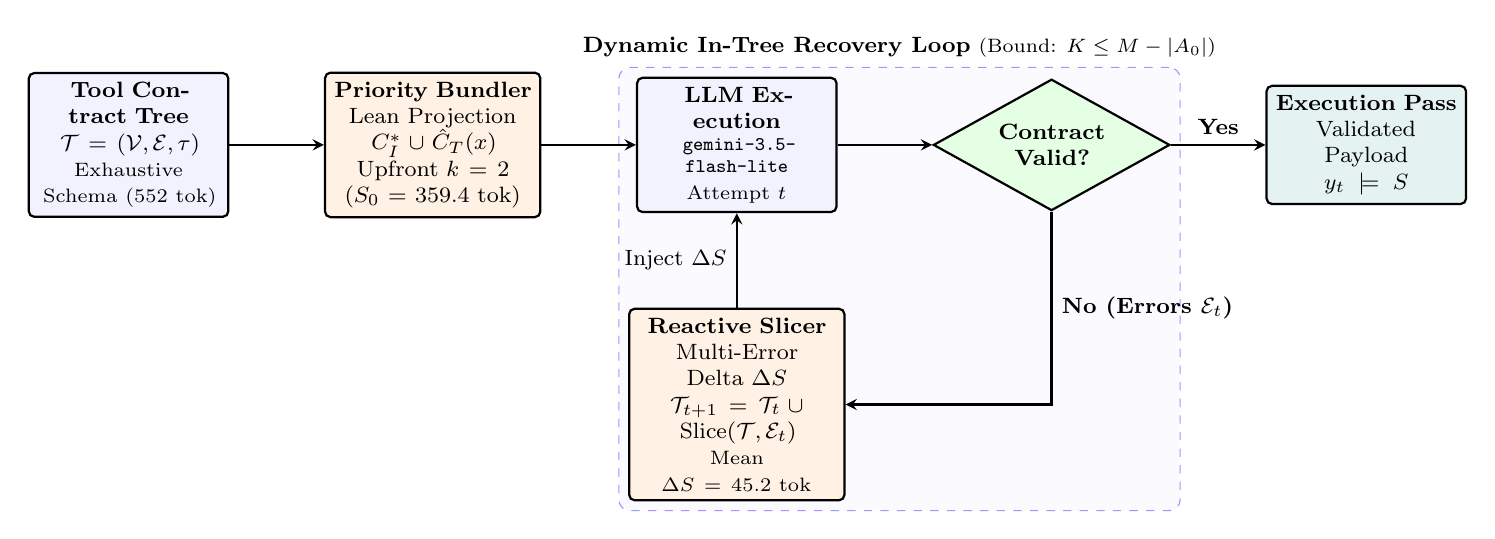
\begin{tikzpicture}[
    node distance=1.4cm and 1.2cm,
    block/.style={rectangle, draw=black, thick, fill=blue!5, text width=2.3cm, text centered, rounded corners=2pt, minimum height=1.1cm, font=\footnotesize},
    process/.style={rectangle, draw=black, thick, fill=orange!10, text width=2.5cm, text centered, rounded corners=2pt, minimum height=1.1cm, font=\footnotesize},
    decision/.style={diamond, draw=black, thick, fill=green!10, text width=1.4cm, text centered, aspect=1.8, font=\footnotesize},
    output/.style={rectangle, draw=black, thick, fill=teal!10, text width=2.3cm, text centered, rounded corners=2pt, minimum height=1.1cm, font=\footnotesize},
    line/.style={draw=black, -stealth, thick},
    dashline/.style={draw=black, -stealth, thick, dashed}
]

% Nodes
\node [block] (input) {\textbf{Tool Contract Tree}\\ $\mathcal{T} = (\mathcal{V}, \mathcal{E}, \tau)$ \\ \scriptsize Exhaustive Schema (552 tok)};

\node [process, right=of input] (bundler) {\textbf{Priority Bundler}\\ Lean Projection $C_I^* \cup \hat{C}_T(x)$\\ Upfront $k=2$ ($S_0=359.4$ tok)};

\node [block, right=of bundler] (llm) {\textbf{LLM Execution}\\ \scriptsize\texttt{gemini-3.5-}\\ \scriptsize\texttt{flash-lite}\\ Attempt $t$};

\node [decision, right=of llm] (val) {\textbf{Contract}\\ \textbf{Valid?}};

\node [output, right=of val] (success) {\textbf{Execution Pass}\\ Validated Payload\\ $y_t \models S$};

\node [process, below=1.2cm of llm] (slicer) {\textbf{Reactive Slicer}\\ Multi-Error Delta $\Delta S$\\ $\mathcal{T}_{t+1} = \mathcal{T}_t \cup \text{Slice}(\mathcal{T}, \mathcal{E}_t)$\\ \scriptsize Mean $\Delta S = 45.2$ tok};

% Paths
\path [line] (input) -- (bundler);
\path [line] (bundler) -- (llm);
\path [line] (llm) -- (val);
\path [line] (val) -- node[above, font=\footnotesize\bfseries] {Yes} (success);
\path [line] (val) |- node[right, font=\footnotesize\bfseries, near start] {No (Errors $\mathcal{E}_t$)} (slicer);
\path [line] (slicer) -- node[left, font=\footnotesize] {Inject $\Delta S$} (llm);

% Background box for in-tree recovery
\begin{scope}[on background layer]
    \node [draw=blue!40, dashed, fill=blue!2, rounded corners=4pt, fit=(llm) (val) (slicer), label=above:{\footnotesize\textbf{Dynamic In-Tree Recovery Loop} \scriptsize(Bound: $K \le M - |A_0|)$}] {};
\end{scope}

\end{tikzpicture}%
}
\caption{System Architecture of LASR-MCP: The full tool contract tree $\mathcal{T}$ is structurally projected into an invariant foundation $C_I^*$ with $k=2$ prioritized constraint bundles ($S_0 = 359.4$ tokens). Upon validation failure, the reactive slicer dynamically splices concurrent violated constraint subtrees ($\Delta S = 45.2$ tokens) corresponding to the diagnostic error set $\mathcal{E}_t$ into Attempt $t+1$, bounded by the monotonic convergence invariant $K \le M - |A_0|$.}
\label{fig:system_architecture}
\end{figure*}


To resolve the trade-off between bloated context overhead and brittle schema truncation, we introduce \textbf{Learned Adaptive Schema Resolution (LASR-MCP)}. Rather than treating tool schemas as static monolithic declarations or appending unanchored constraint slices, LASR-MCP formulates the active tool schema at execution attempt $t$ as a three-tier union:
\begin{equation}
\label{eq:three_tier}
C_{\text{active}}^{(t)} = C_I^* \;\cup\; \hat{C}_T(x) \;\cup\; C_R^{(t)}
\end{equation}
where $C_I^*$ represents the schema-wide \textit{Invariant Foundation}, $\hat{C}_T(x)$ is the \textit{Proactive Task-Conditioned Constraint Bundle} predicted from user intent $x$, and $C_R^{(t)}$ is the accumulated set of \textit{Dynamically Recovered In-Tree Constraints} derived from validation feedback up to round $t$.

\subsection{Tier 1: Invariant Foundation Floor ($C_I^*$)}
Empirical inspection of complex JSON Schema specifications (e.g., enterprise purchase order dispatching) reveals that tool execution cannot succeed on intent-specific properties alone. Certain structural constraints are \textit{invariants} required for all syntactically well-formed submissions regardless of user goal (e.g., supplier identification regex format, item array container specifications, and SKU patterns).

Let $\mathcal{C}_{\text{full}}$ denote the complete schema constraint set ($552$ tokens). We define the Invariant Foundation $C_I^*$ as the minimal constraint subset among tested candidates satisfying the pre-specified baseline structural-validity floor without user-intent conditioning:
\begin{equation}
C_I^* = \arg\min_{C \in \mathcal{C}_{\text{cand}}} |C| \quad \text{s.t.} \quad \mathcal{V}_{\text{struct}}(C) \ge \tau_{\text{floor}}
\end{equation}
where $\mathcal{C}_{\text{cand}}$ is the set of evaluated candidate invariant subsets and $\tau_{\text{floor}} = 0.70$ specifies the baseline validity floor, chosen \textit{a priori} as the minimum operational viability threshold to avoid retry cascade failure. As demonstrated in Section~\ref{sec:results}, $C_I^* = 339$ tokens is the empirically selected invariant foundation meeting this threshold among tested tiers for the evaluated purchase-order schema; compressing below this boundary triggers structural collapse in nested item definitions.

\subsection{Tier 2: Proactive Intent-Conditioned Predictor ($\hat{C}_T(x)$)}
Given a user query $x \in \mathcal{X}$, the agent's goal is to predict the minimal subset of task-conditioned constraints $\hat{C}_T(x) \subseteq \mathcal{C}_{\text{task}}$ necessary for successful execution. We formulate this as a multi-label classification problem over the task-conditioned label space $\mathcal{L} = \{c_1, c_2, \dots, c_m\}$ (e.g., specific warehouse routing enums, order priority restrictions, and budget bounds).

We employ a frozen linear semantic predictor:
\begin{equation}
\hat{y}_i = \sigma\left( \mathbf{w}_i^T \phi(x) + b_i \right), \quad i \in \{1, \dots, m\}
\end{equation}
where $\phi(x)$ denotes normalized term-salience features extracted from the query. The decision threshold $\theta$ was calibrated strictly on the 48 training tasks and frozen prior to evaluation. To construct the proactive bundle of size up to $k$, the highest-ranked constraints exceeding $\theta$ (up to $k$) are selected:
\begin{equation}
\hat{C}_T(x) = \text{Top-}k \left( \{ c_i \in \mathcal{L} \mid \hat{y}_i \ge \theta \} \right)
\end{equation}
We formally denote by $m_{\text{task}}(x) = |C_T^*(x)|$ the number of required non-invariant task-conditioned constraints demanded by user intent $x$. The condition $m_{\text{task}}(x) \le k$ is an operational regime descriptor characterizing when task requirements do not exceed the upfront budget capacity $k$, rather than a guarantee that the heuristic predictor selects all required constraints on Attempt 1 (e.g., in Cluster $C_1$, first-pass hierarchical success is $75.0\%$, though final structural success recovers to $100.0\%$). Conversely, $m_{\text{task}}(x) > k$ defines regimes where omissions are structurally guaranteed.

\subsection{Tier 3: Dynamic In-Tree Recomposition ($C_R^{(t)}$)}
\label{sec:recomposition}
When an unpredicted constraint is omitted from $C_I^* \cup \hat{C}_T(x)$, the LLM may submit arguments $y_t$ that fail JSON Schema validation. A simple agent implementation may return raw validator error strings into conversation history or retry without modifying the exposed schema. 

LASR-MCP introduces \textit{in-tree reactive recomposition}. Reactive recovery operates as pass-level multi-error constraint expansion rather than single-error sequential repair. Our validator is configured to return all observed violations $\text{Errors}(y_t) = \{e_1, e_2, \dots\}$ in a single validation pass, rather than short-circuiting on the first failure. Analogous to an enterprise validator reporting all diagnostic issues across a payload, the reactive operator extracts all concurrent violations simultaneously:
\begin{equation}
\label{eq:reactive_op}
C_R^{(t+1)} = C_R^{(t)} \cup \bigcup_{e \in \text{Errors}(y_t)} \left( \text{Fragment}(e) \cap \mathcal{S}_{\text{specs}} \setminus C_{\text{active}}^{(t)} \right)
\end{equation}
where $\text{Fragment}(e)$ deterministically maps the RFC 6901 JSON Pointer error path~\cite{rfc6901} and validator-reported JSON Schema keyword (e.g., \texttt{path='/warehouse\_code'}, \texttt{keyword='enum'}) to the canonical constraint node $\Delta_e \in \mathcal{S}_{\text{specs}}$.

The updated schema specification $S_{t+1}$ is then structurally spliced into the native JSON Schema hierarchy:
\begin{equation}
S_{t+1} = \mathcal{R}\left( S_I, C_{\text{active}}^{(t+1)} \right)
\end{equation}
where $\mathcal{R}$ is the in-tree recomposition function that inserts properties, pattern regexes, and enums directly into their respective object trees without creating duplicate definition nodes or schema syntax errors.

\subsection{Incremental Token Accounting Metrics}
To evaluate token economics, we audit token consumption at every turn:
\begin{itemize}
    \item \textbf{Initial Schema Overhead ($S_0$)}: Tokens required to serialize $S_{\text{active}}^{(1)}$.
    \item \textbf{Incremental Expansion ($\Delta S_t$)}: Additional schema tokens introduced at attempt $t \ge 2$: $\Delta S_t = \text{Tok}(S_t) - \text{Tok}(S_{t-1})$.
    \item \textbf{Structural Tokens-to-Success ($\text{TTS}_{\text{struct}}$)}: Cumulative recorded prompt-plus-candidate tokens across all attempts conditional on structurally successful trajectories ($y_{T_{\text{succ}}} \models \mathcal{S}$ within attempt budget $T_{\text{succ}} \le 3$):
    \begin{equation}
    \begin{split}
    TTS_{\text{struct}} &= \sum_{t=1}^{T_{\text{succ}}} \text{Recorded } (P+C)_t \\
    &= \sum_{t=1}^{T_{\text{succ}}} \bigl( \texttt{promptTokenCount}_t \\
    &\qquad\quad + \texttt{candidatesTokenCount}_t \bigr)
    \end{split}
    \end{equation}
    where provider-recorded prompt tokens natively encompass both non-schema text ($P_t$) and the serialized active schema ($\text{Tok}(S_t)$), preventing offline double-counting, while $C_t$ represents candidate completion tokens.
    \item \textbf{Total Workload Tokens}: Sum of all tokens consumed across all attempts up to the three-attempt budget, including failed retry loops. We explicitly distinguish total workload on the historical development benchmark (32 unique task trials per arm) from the canonical live benchmark (640 task executions per arm across 20 fixed-seed repetitions; 3,840 total trials across all six arms).
    \item \textbf{Structural Recovery Rate}: Fraction of initially structurally invalid trajectories that subsequently satisfy JSON Schema validation within the attempt budget.
\end{itemize}
For workload-token reporting, we use the provider-recorded prompt-plus-candidate token subtotal per request ($\text{Recorded } P+C = \texttt{promptTokenCount} + \texttt{candidatesTokenCount}$, which identically equals provider \texttt{totalTokenCount} across all 7,860 response-bearing calls in our benchmark dataset as thinking and client-side tool prompt tokens are zero; we report this as an audited property of our experimental telemetry rather than an invariant across all API features). Serialized schema tokens ($S_0, \Delta S$) are audited separately as structural diagnostics without double-counting them into provider prompt totals.

\subsection{Formal Foundation \& Invariant Termination Bound}
\label{sec:formal_proof}

Let $\mathcal{S}$ denote a canonical tool specification expressed in JSON Schema Draft 2020-12, represented as an abstract syntax tree (AST). We define $\mathcal{C} = \{c_1, c_2, \dots, c_M\}$ as the finite universe of structural constraint nodes in $\mathcal{S}$ ($|\mathcal{C}| = M = M_{\text{schema}} < \infty$), where each constraint node $c_i$ corresponds to an unambiguous validation keyword (e.g., \texttt{pattern}, \texttt{enum}, \texttt{minimum}, \texttt{required}) situated at a specific JSON Pointer path. We explicitly distinguish this total schema universe size $M_{\text{schema}}$ from task-conditioned constraint requirements $m_{\text{task}}(x)$.

The reactive framework operates over a sequence of active constraint sets $A_t \subseteq \mathcal{C}$ at recovery step $t \ge 0$, initialized as $A_0 = C_I^* \cup \widehat{C}_T(x)$. At step $t$, the generator outputs argument payload $y_t$. If $y_t$ violates schema constraints, the validator returns diagnostics $\mathcal{E}(y_t, \mathcal{S}) \neq \emptyset$. The deterministic slicer $\sigma$ maps each diagnostic to its canonical schema constraint node. To ensure strict non-redundant growth, the newly identified constraint delta is defined by explicitly filtering previously active nodes:
\begin{equation}
\Delta_t = \left( \bigcup_{e \in \mathcal{E}(y_t, \mathcal{S})} \sigma(e, \mathcal{S}) \right) \setminus A_t
\end{equation}
The reactive recomposer then updates the active constraint set in-tree: $A_{t+1} = A_t \cup \Delta_t$.

\begin{definition}[Admissible Reactive System]
A reactive tool-calling system $(\mathcal{S}, \sigma, \mathcal{G})$ is admissible if:
\begin{enumerate}
    \item \textbf{Finite Constraint Universe}: The schema AST contains a finite number of constraint nodes, $|\mathcal{C}| = M = M_{\text{schema}} < \infty$.
    \item \textbf{Non-Empty Fault Localization}: On any validation failure at step $t$, the slicer identifies at least one previously inactive constraint: $|\Delta_t| \ge 1$ and $\Delta_t \cap A_t = \emptyset$.
    \item \textbf{Strict Monotonicity}: Each localized constraint is merged idempotently without pruning active constraints, ensuring $A_t \subset A_{t+1} \subseteq \mathcal{C}$.
\end{enumerate}
\end{definition}

\begin{theorem}[Finite Monotonic Recovery Bound]
\label{thm:termination}
Let $(\mathcal{S}, \sigma, \mathcal{G})$ be an admissible reactive tool-calling system with initial active constraint set $A_0 \subseteq \mathcal{C}$ and full schema universe $M_{\text{schema}} = |\mathcal{C}| = M$. The dynamic in-tree recovery process terminates in at most:
\begin{equation}
\boxed{K \le M - |A_0|}
\end{equation}
schema-expansion transitions (where $M \equiv M_{\text{schema}}$), resulting in either a structurally valid payload or complete exhaustion of the schema ($A_K = \mathcal{C}$).
\end{theorem}

\begin{IEEEproof}
By the non-empty fault localization condition, whenever $y_t$ is invalid, $\Delta_t \subseteq \mathcal{C} \setminus A_t$ and $|\Delta_t| \ge 1$. Consequently:
\begin{equation}
|A_{t+1}| = |A_t \cup \Delta_t| = |A_t| + |\Delta_t| \ge |A_t| + 1
\end{equation}
Thus, the active cardinality sequence is strictly monotonically increasing: $|A_0| < |A_1| < \dots < |A_K| \le M$. By induction across $K$ transitions, $|A_K| \ge |A_0| + K$. Because $|A_K| \le M$, it follows directly that $|A_0| + K \le M \implies K \le M - |A_0|$. Because $\mathcal{C}$ is finite and omitted constraints strictly decrease, the recovery loop cannot cycle or run indefinitely, guaranteeing termination in at most $M - |A_0|$ transitions.
\end{IEEEproof}
We emphasize that Theorem~\ref{thm:termination} bounds dynamic schema expansion under its stated admissibility conditions; it guarantees that the active schema contract monotonically expands to full specification in at most $M - |A_0|$ transitions, but does not guarantee that a stochastic model will always generate a valid payload if the model violates already-exposed constraints or if execution is constrained by an operational attempt budget (such as $T_{\text{max}} = 3$).

\begin{remark}[Analysis of the Invalid Tree-Depth Bound $K \le D$]
Earlier heuristic drafts proposed a bound of $K \le \min(D, M - |C_I^*|)$, where $D$ represents maximum AST depth. This claim does not hold in general. Consider two sibling leaf constraints at depth $D = 1$: $c_1 =$ \texttt{properties/warehouse\_code/enum} and $c_2 =$ \texttt{properties/order\_priority/enum}. On Attempt 1 ($A_0 = \emptyset$), the generator may violate $c_1$ (splicing $c_1$). On Attempt 2, it may satisfy $c_1$ but violate $c_2$ (splicing $c_2$), converging on Attempt 3. This yields $K = 2$ transitions even though $D = 1$. Since $2 \not\le 1$, tree depth does not constrain recovery passes. Theorem~\ref{thm:termination} establishes the correct cardinality-based bound.
\end{remark}

\begin{proposition}[Structural Validity Guarantee]
If the generator $\mathcal{G}$ satisfies the \emph{exposed-constraint compliance assumption}---namely, that $\mathcal{G}$ satisfies all constraints in $A_t$ and failures arise strictly from omitted constraints in $\mathcal{C} \setminus A_t$---then the recovery loop terminates with a structurally valid invocation ($y_K \models \mathcal{S}$) in $K \le M - |A_0|$ transitions.
\end{proposition}

\begin{remark}[Deterministic Schema Convergence vs.\ Stochastic Decoding Adherence]
It is critical to distinguish between \emph{deterministic schema state convergence} and \emph{stochastic LLM decoding adherence}. Theorem~\ref{thm:termination} guarantees that the schema contract itself strictly and monotonically expands to include all violated constraints within at most $M - |A_0|$ steps. However, once a constraint is exposed in the prompt, actual generative compliance depends on the model's stochastic decoding adherence. In our live $N=3,840$ empirical evaluation on \texttt{gemini-3.5-flash-lite}, this distinction accounts for the observed $96.9\%$ vs.\ $100.0\%$ final structural completion rate: the schema state monotonically reached full specification, but the model occasionally generated invalid edge-case syntax on Attempt 3 in complex multi-item nested arrays ($C_3$).
\end{remark}



\section{Experimental Setup}
\label{sec:setup}

\subsection{Task Corpus \& Stratified Template Splits}
We evaluate LASR-MCP on a synthetic enterprise-style supply-chain tool execution benchmark (\texttt{create\_purchase\_order}) governing multi-item warehouse replenishment. The benchmark corpus comprises 80 pre-specified task instances partitioned strictly across syntactic template families:
\begin{itemize}
    \item \textbf{Training Tasks ($N=48$)}: Derived from template families \texttt{family\_a} and \texttt{family\_b}, used to train the frozen semantic predictor.
    \item \textbf{Evaluation Tasks ($N=32$)}: Drawn exclusively from \texttt{family\_c} with distinct lexical and syntactic structures (serving as unseen held-out test tasks for $H_1$ intent prediction, and development/validation tasks for $H_2$--$H_4$ systems evaluation).
\end{itemize}
The 32 evaluation tasks span four diverse operational archetypes ($N=8$ tasks each):
\begin{enumerate}
    \item \textbf{C1: Routine Regional Replenishment}: High-frequency, standard priority orders governed by basic warehouse routing.
    \item \textbf{C2: Expedited Emergency Orders}: Critical priority dispatches with accelerated freight logistics and rigid budget limits.
    \item \textbf{C3: Specialized Bulk Procurement}: Large-quantity orders where queries omit explicit warehouse locations, testing model behavior under unstated default enums.
    \item \textbf{C4: Multi-Item Depot Rebalancing}: Complex multi-line consignments enforcing nested \texttt{maxItems} and item-level SKU validation.
\end{enumerate}

\subsection{Controlled Experimental System Arms}
To compare the contributions of the schema-resolution components in Equation~\eqref{eq:three_tier}, we evaluate six controlled system arms under identical prompt conditions:
\begin{itemize}
    \item \textbf{Full Schema Control (\texttt{full})}: Static exposure of the monolithic 552-token schema upfront.
    \item \textbf{Invariant Baseline (\texttt{ci\_k0})}: Invariant Foundation alone ($C_I^* = 339$ tokens) without task-conditioned prediction or reactive recovery.
    \item \textbf{Proactive Static Control (\texttt{ci\_k1\_static})}: Invariant Foundation + Top-1 LASR predicted constraint without reactive recovery.
    \item \textbf{Proactive-Reactive LASR (\texttt{ci\_k1\_reactive})}: Invariant Foundation + Top-1 LASR predicted constraint with dynamic in-tree recovery.
    \item \textbf{Proactive-Reactive LASR (\texttt{ci\_k2\_reactive})}: Invariant Foundation + Top-2 LASR predicted constraints with dynamic in-tree recovery.
    \item \textbf{Model-Conditional Reference (\texttt{oracle\_reactive})}: Invariant Foundation + reference constraint set $O(x) = C_I^* \cup C_T^*(x)$ with reactive recovery. $O(x)$ was constructed from task specifications prior to execution and validated against the schema validator.
\end{itemize}

\subsection{Dual Evaluation Criteria \& Metric Definitions}
Submissions are evaluated on two orthogonal metrics alongside token efficiency:
\begin{enumerate}
    \item \textbf{Structural Schema Validity (\%)}: Conformance to JSON Schema Draft 2020-12 verified by an independent automated validator.
    \item \textbf{Semantic Task Correctness (\%)}: Exact domain logic validation verifying that extracted line items, quantities, priority codes, and supplier IDs satisfy user intent. Evaluation is strictly hierarchical: semantic correctness requires structural validity as a precondition ($\text{First-Pass Hierarchical} = \text{Structural} \land \text{Semantic}$), bounding semantic correctness by structural success.
    \item \textbf{Recorded Token Metric \& Accounting Reconciliation}: The primary token metric is defined strictly as the provider-recorded prompt-plus-candidate token subtotal per recorded attempt:
    \begin{equation}
    \text{Recorded } P+C = \text{prompt\_tokens} + \text{completion\_tokens}
    \end{equation}
    directly derived from Google's \texttt{usageMetadata} (\texttt{promptTokenCount} + \texttt{candidatesTokenCount}, which identically equals provider \texttt{totalTokenCount} across all 7,860 calls in our benchmark dataset as thinking and client tool prompt tokens are zero). In earlier preliminary benchmark drafts, heuristic offline schema token estimates ($S_0 + \Delta S$) were inadvertently added to provider prompt tokens, creating an artificial double-counting distortion that heavily penalized Full Control (whose monolithic schema is already serialized inside the prompt). In v2.0.3, we eliminate this double-counting artifact entirely: heuristic schema sizes ($S_0, \Delta S$) are decoupled and retained strictly as offline structural diagnostics, while all economic and token workload evaluations rely exclusively on provider-reported $P+C$ token usage from \texttt{usageMetadata}.
\end{enumerate}

\subsection{Execution Environment \& Live Telemetry Ledger}
All live experiments were executed against model ID \texttt{gemini-3.5-flash-lite} hosted on Google Cloud Generative Language API via direct REST HTTP endpoints. The provider telemetry explicitly records \texttt{requested\_model} and \texttt{provider\_resolved\_model\_version} as \texttt{gemini-3.5-flash-lite} (returned in the API \texttt{modelVersion} field); the API reported this model alias directly, and a separate immutable backend snapshot tag was not exposed by the endpoint. In our client configuration, \texttt{LiveLLMClient} operated at temperature $0.2$, and requests transmitted a fixed execution seed (\texttt{seed=42}). Across the 20 repeated executions per task-arm combination, the model produced deterministic identical first responses and outcomes under the repeated fixed seed; the 32 distinct task IDs represent the paired resampling units of inference, and the 20 replicates verify execution determinism under fixed decoding conditions rather than representing independent stochastic draws. 

The live empirical dataset comprises exactly $N=3,840$ completed trials across the 32 tasks and 6 experimental arms, producing $7,860$ response-bearing provider calls (all HTTP 200, with 100\% complete provider \texttt{usageMetadata} recording \texttt{promptTokenCount}, \texttt{candidatesTokenCount}, and \texttt{totalTokenCount}). Transient network rate limits (HTTP 429 and 503) triggered exactly 154 client transport retries; these transport-level backoffs are cleanly isolated and reported separately from logical agent attempts. 

We distinguish the full multi-session data collection timeline from the duration of the final resumed session: the total collection spanned multiple days across paid and quota-limited API sessions, completing 3,149 trials in initial sessions followed by a final resumed session completing the remaining 691 trials in approximately 2.8 hours. Operational execution ledgers are preserved in the reproducibility archive.

\subsection{Statistical Inference: Paired Task-Cluster Percentile Bootstrap}
For all comparative workload evaluations between experimental arms, we employ a paired task-cluster percentile bootstrap over the 32 task clusters. The 32 distinct task IDs constitute the resampling units of inference. For each bootstrap iteration ($B=10,000$ resamples, deterministic seed 42), task clusters are sampled with replacement, computing paired workload differences and cluster-level ratios. Confidence intervals are reported as empirical 2.5\% and 97.5\% percentiles of the bootstrap distribution.

\subsection{Evaluation Hygiene \texorpdfstring{\&}{and} Benchmark Scope}
To maintain strict methodological hygiene, we explicitly delineate the empirical role of each benchmark split:
\begin{itemize}
    \item \textbf{Held-Out Family Generalization for $H_1$}: The intent-conditioned predictor is implemented as a custom multi-label log-odds-weighted lexical classifier with class priors and smoothed IDF weights. It was trained on 48 tasks (\texttt{family\_a}, \texttt{family\_b}) and evaluated on 32 tasks (\texttt{family\_c}) drawn from a held-out syntactic template family. While template framing structures are strictly partitioned, shared enterprise procurement vocabulary exists across splits (103 of 149 test vocabulary words, $69.1\%$ overlap), and all four target constraint combinations recur across train and test families. Predictor weights were formally frozen prior to all systems evaluations.
    \item \textbf{Primary Frozen Benchmark for $H_2$--$H_4$}: The invariant foundation $C_I^* = 339$ tokens was calibrated on an 8-task calibration probe (\texttt{BLIND-C1-013}, \texttt{BLIND-C1-014}, \texttt{BLIND-C2-013}, \texttt{BLIND-C2-014}, \texttt{BLIND-C3-013}, \texttt{BLIND-C3-014}, \texttt{BLIND-C4-013}, \texttt{BLIND-C4-014}) sampled directly from the \texttt{family\_c} task distribution (two tasks per cluster). Consequently, the 8-task probe overlaps the 32 evaluation tasks; we explicitly disclose this tuning/evaluation overlap and evaluate $H_2$--$H_4$ as characterizing systems behavior within this primary frozen benchmark corpus rather than serving as an untouched, blind end-to-end generalization test.
\end{itemize}

\subsection{Data Provenance \texorpdfstring{\&}{and} Trace Replay Verification}
All benchmark code, traces, and frozen datasets are archived at \url{https://github.com/AnandSuchak/mcp-inventory-bench}. While live API re-executions may exhibit variance from hosted model updates, recorded execution traces support deterministic replay of the reported experiments, verified by automated cryptographic manifests:
\begin{center}
\footnotesize
\textbf{Cryptographic Artifact Provenance:}\\
\textit{Frozen Benchmark ($N=32$):}\\
\texttt{\scriptsize SHA-256: 78c2c88ed5128e0f296fa29e0c258589}\\
\texttt{\scriptsize \phantom{SHA-256: }b516f3adb14b0b8da491fa73bc3ffc11}\\
\textit{v2.0.3 Live Benchmark Candidate ($N=3,840$):}\\
\texttt{\scriptsize SHA-256: fc82d33b8992914ee130ef2805427ef2}\\
\texttt{\scriptsize \phantom{SHA-256: }a4f01541243e0f93be120e2d20ae7f5b}\\
\texttt{\scriptsize Commit: 9807340abc38170e0090a102547ee4309c01d78b}
\end{center}
Automated regression test suites ensure complete data immutability.


\section{Empirical Results \texorpdfstring{\&}{and} Discussion}
\label{sec:results}

We structure our empirical analysis around four core research hypotheses evaluated across the primary 32-task frozen benchmark corpus.

\subsection{$H_1$: Semantic Predictability over Frequency Baselines}
We first evaluate whether intent-driven multi-label classification can reliably anticipate task-conditioned constraints on unseen template families compared to an empirical frequency prior. The frequency prior ranks constraint labels by empirical prevalence across the 48 training tasks and selects the top-$k$ most frequent constraints.
On the unseen template family evaluation ($N=32$ from \texttt{family\_c}), LASR's custom log-odds lexical classifier at $k=2$ achieves an $F_1$ score of \textbf{0.863} (exact mean $0.8625$) and a \textbf{68.8\% exact bundle match} ($22/32$ tasks), compared to \textbf{$F_1 = 0.250$} and $25.0\%$ exact match ($8/32$ tasks) for the Frequency Prior baseline. Resampling the 32 evaluation tasks with replacement for $B=10,000$ paired task-level bootstrap replicates (seed 42) and evaluating a Monte Carlo one-sided paired sign-flip permutation test ($B=10,000$ draws, seed 42) with valid $(k+1)/(B+1)$ correction yields:
\begin{equation}
\Delta F_1 = \mathbf{+0.613} \quad [95\% \text{ CI: } +0.419, +0.781], \quad p < 0.001
\end{equation}
(exact unrounded $\Delta F_1 = +0.6125$, bootstrap interval $[0.4188, 0.7812]$, Monte Carlo $p = (0+1)/(10000+1) \approx 0.0001$). While template syntax was partitioned across families, shared enterprise procurement terminology accounts for a 69.1\% test vocabulary overlap (103/149 words), and all 4 target constraint combinations recur across train and test sets.

\noindent\textbf{Cluster-Dependence Sensitivity Analysis}: As a sensitivity check across semantic domains, equal-weighting the four cluster mean $F_1$ differences ($N=4$ clusters, 8 tasks each) yields an equal-weighted delta $+0.613$ ($+0.6125$) with exhaustive four-cluster sign-flip permutation $p = 2/16 = 0.125$. Similarly, testing cluster-level reactive-vs-static structural gains yields an equal-weighted lift of $+21.9\text{ pp}$ ($p = 0.125$). While task-level paired differences are statistically consistent across the 32 individual tasks ($p < 0.001$), inference across cluster archetypes is limited by the sample of four semantic clusters with recurring target constraint combinations. We therefore interpret $H_1$ as confirming reliable intent-conditioned prediction on this held-out template family, rather than demonstrating unbounded semantic generalization to arbitrary unseen constraint combinations.

\begin{table*}[t]
\centering
\caption{Initial Single-Trial Frozen Benchmark Systems Evaluation ($N=32$ Tasks, Gemini 3.5 Flash-Lite)}
\label{tab:systems_evaluation}
\resizebox{\textwidth}{!}{%
\begin{tabular}{lcccccccc}
\toprule
\textbf{System Arm} & \textbf{Reactive?} & \textbf{Init $S_0$} & \textbf{Exp. $\Delta S$} & \textbf{1st-Pass Hier. (\%)} & \textbf{Struct. (\%)} & \textbf{Sem. (\%)} & \textbf{Mean $TTS_{\text{P+C}}$} & \textbf{Recorded P+C Tokens} \\
\midrule
Full Schema Control (\texttt{full}) & No & 552.0 & 0.0 & 31.3\% & \textbf{93.8\%} & 90.6\% & 1864.4 & \textbf{61,853} \\
$C_I^*$ Baseline (\texttt{ci\_k0}, $k=0$) & No & 339.0 & 0.0 & 0.0\% & 68.8\% & 65.6\% & 2196.7 & 70,541 \\
LASR Static (\texttt{ci\_k1\_static}, $k=1$) & No & 361.1 & 0.0 & 15.6\% & 78.1\% & 71.9\% & 1631.0 & 56,947 \\
LASR Reactive (\texttt{ci\_k1\_reactive}, $k=1$) & Yes & 361.1 & 45.4 & 15.6\% & \textbf{100.0\%} & 93.8\% & 1612.3 & 51,594 \\
LASR Reactive (\texttt{ci\_k2\_reactive}, $k=2$) & Yes & 366.8 & 43.8 & 18.8\% & \textbf{100.0\%} & 93.8\% & 1571.1 & \textbf{50,276} \\
Oracle Reference* (\texttt{oracle\_reactive}) & Yes & 359.0 & 48.3 & 15.6\% & 96.9\% & 93.8\% & 1554.0 & 50,578 \\
\bottomrule
\end{tabular}%
}
\vspace{1mm}
\begin{minipage}{\textwidth}
\footnotesize
*\textit{Note}: Oracle $O(x)$ is a model-conditional reference baseline. 1st-Pass Hierarchical success requires both structural validity and semantic correctness on Attempt 1 (Full Schema: 10/32 tasks, 31.25\%, displayed 31.3\%). Mean $TTS_{\text{P+C}}$ is the average recorded prompt-plus-candidate token subtotal over structurally successful trajectories ($N_{\text{succ}}$); Recorded P+C Tokens accounts for all prompt and completion tokens across all attempts without heuristic schema double-counting.
\end{minipage}
\end{table*}


\begin{figure*}[t]
\centering
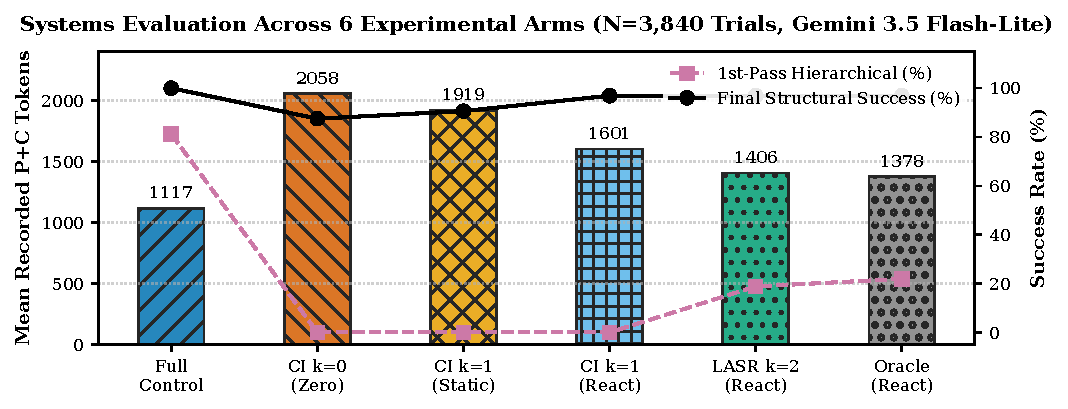
\includegraphics[width=\textwidth]{figures/fig2_systems_evaluation.pdf}
\caption{Systems Evaluation across 6 Experimental Arms ($N=3,840$ Live Trials, \texttt{gemini-3.5-flash-lite}). Bars denote Mean Recorded $P+C$ Tokens per trial; lines denote 1st-Pass Hierarchical Success (\%) and Final Structural Success (\%). Prioritized upfront bundling ($k=2$) slashes token waste by $31.7\%$ vs.\ naive lean schemas ($k=0$) and recovers $96.9\%$ final structural completion.}
\label{fig:systems_evaluation_6arms}
\end{figure*}

\subsection{$H_2$: Invariant Foundation Requirement on the Evaluated Benchmark}
To identify the minimal invariant floor $C_I^*$ meeting the pre-specified 70\% structural-validity threshold ($\tau_{\text{floor}} = 0.70$), we followed a formal sequential design: \textit{pre-specify threshold} $\rightarrow$ \textit{candidate calibration} $\rightarrow$ \textit{freeze $C_I^*$} $\rightarrow$ \textit{final 32-task systems evaluation}.
During candidate calibration on an 8-task calibration probe (\texttt{BLIND-C1-013}, \texttt{BLIND-C1-014}, \texttt{BLIND-C2-013}, \texttt{BLIND-C2-014}, \texttt{BLIND-C3-013}, \texttt{BLIND-C3-014}, \texttt{BLIND-C4-013}, \texttt{BLIND-C4-014}, sampled directly from the 32 evaluation tasks as disclosed in Section~\ref{sec:setup}-F), we benchmarked three candidate compression tiers prior to task conditioning:
\begin{itemize}
    \item \textbf{Tier 1 (Standard $C_I^*$, 339 tokens)}: 75.0\% structural validity (6/8 tasks).
    \item \textbf{Tier 2 (Compact $C_I$, 308 tokens)}: 62.5\% structural validity (5/8 tasks).
    \item \textbf{Tier 3 (Minimal $C_I$, 284 tokens)}: 50.0\% structural validity (4/8 tasks).
\end{itemize}
Tier 1 ($C_I^* = 339$ tokens) was the smallest tested candidate meeting the 70\% floor and was frozen for all subsequent experiments.
In the subsequent full 32-task systems benchmark (Table~\ref{tab:systems_evaluation}), this frozen foundation alone without task prediction (\texttt{ci\_k0}) yielded 68.8\% structural validity (22/32 tasks), confirming that without task-conditioned augmentation or reactive recovery, structural validity hovers near the 70\% baseline floor. Compressing below 339 tokens triggers progressive degradation due to missing definitions for nested items. We emphasize that 339 tokens represents the smallest tested candidate meeting this threshold, not an unconstrained universal constant.

\subsection{$H_3$: Structural Contribution of Reactive In-Tree Recovery}
\begin{table}[htbp]
\centering
\caption{Historical Paired Differences and Hypothesis Tests ($N=32$ Single-Trial Development Benchmark)}
\label{tab:paired_bootstrap}
\setlength{\tabcolsep}{2.5pt}
\resizebox{\columnwidth}{!}{%
\begin{tabular}{lccccc}
\toprule
\textbf{Pairwise Contrast} & \textbf{Metric} & \textbf{Point Est.} & \textbf{95\% CI} & \textbf{Token Diff.} & \textbf{Statistical Method} \\
\midrule
LASR Reactive vs Static ($k=1$) & $\Delta$ Structural Succ. & \textbf{+21.9 pp} & [9.4, 37.5] pp & --- & Exact McNemar ($p = 0.0078125$) \\
& $\Delta$ Semantic Corr. & \textbf{+21.9 pp} & [9.4, 37.5] pp & --- & Exact McNemar ($p = 0.0078125$) \\
\midrule
LASR Reactive ($k=1$) vs Full & $\Delta$ Structural Succ. & +6.3 pp & [0.0, 15.6] pp & --- & Exact McNemar ($p = 0.250$) \\
& $\Delta$ Semantic Corr. & +3.1 pp & [-6.3, 15.6] pp & --- & Exact McNemar ($p = 0.500$) \\
\midrule
LASR Reactive ($k=1$) vs Full & Signed Token Savings & \textbf{+16.6\%} & --- & -10,259 tokens & Total Token Diff (No CI) \\
LASR Reactive ($k=2$) vs Full & Signed Token Savings & \textbf{+18.7\%} & --- & -11,577 tokens & Total Token Diff (No CI) \\
\bottomrule
\end{tabular}%
}
\end{table}

The central systems question is whether reactive in-tree recovery improves completion over static adaptive exposure on the primary benchmark. In Table~\ref{tab:systems_evaluation}, we contrast \texttt{ci\_k1\_static} directly with \texttt{ci\_k1\_reactive}:

\noindent\textbf{Structural Reliability}: Final structural success increases from \textbf{78.1\%} to \textbf{100.0\%} ($\Delta\text{Success} = \mathbf{+21.9\text{ pp}}$, 95\% CI: $[+9.4, +37.5]\text{ pp}$, exact one-sided McNemar/binomial test $p = 0.0078125$; cluster-level sensitivity $p = 0.125$).

\noindent\textbf{Semantic Correctness}: Task correctness increases from \textbf{71.9\%} to \textbf{93.8\%} ($\Delta\text{Correctness} = \mathbf{+21.9\text{ pp}}$, 95\% CI: $[+9.4, +37.5]\text{ pp}$, exact one-sided McNemar/binomial test $p = 0.0078125$).

\noindent\textbf{Structural Recovery Rate}: Under \texttt{ci\_k1\_reactive} on the initial development benchmark ($N=32$), exactly 27 trajectories initially failed structural validation on Attempt~1 ($5/32 = 15.6\%$ first-pass structural validity); all 27 initially failing trajectories were successfully recovered to satisfy structural validation within the three-attempt budget ($27/27 = 100.0\%$ structural recovery; $32/32$ final structural, $30/32$ final semantic). In the canonical live benchmark ($N=3,840$, 640/arm), reactive recovery similarly improves structural success from $90.625\%$ ($580/640$) to $96.875\%$ ($620/640$, $\mathbf{+6.25\text{ pp}}$) and semantic correctness from $87.500\%$ to $93.750\%$ ($\mathbf{+6.25\text{ pp}}$). We report this live comparison alongside the historical $+21.9\text{ pp}$ single-trial benchmark without conflating the two scopes.

As broken down in Table~\ref{tab:cluster_breakdown}, the observed lift is concentrated in Cluster 3 (Specialized Bulk Procurement), where static success was only 50.0\% (4/8 tasks) due to missing warehouse enums, while reactive recovery achieved \textbf{100.0\%} (8/8 tasks).

\begin{table}[htbp]
\centering
\caption{Historical Task Cluster Breakdown: Static Vulnerability vs. Reactive Recovery ($N=32$ Single-Trial Development Benchmark, $N=8$ per Cluster)}
\label{tab:cluster_breakdown}
\setlength{\tabcolsep}{3pt}
\resizebox{\columnwidth}{!}{%
\begin{tabular}{lcccc}
\toprule
\textbf{Task Cluster Archetype} & \textbf{Full (\%)} & \textbf{Static $k=1$} & \textbf{Reactive $k=1$} & \textbf{Reactive vs. Static Lift} \\
\midrule
C1: Routine Regional & 87.5\% & 100.0\% & \textbf{100.0\%} & \textbf{0.0 pp} \\
C2: Expedited Emergency & 100.0\% & 87.5\% & \textbf{100.0\%} & \textbf{+12.5 pp} \\
C3: Specialized Bulk & 87.5\% & 50.0\% & \textbf{100.0\%} & \textbf{+50.0 pp} \\
C4: Multi-Item Depot & 100.0\% & 75.0\% & \textbf{100.0\%} & \textbf{+25.0 pp} \\
\bottomrule
\end{tabular}%
}
\end{table}


\begin{figure*}[t]
\centering
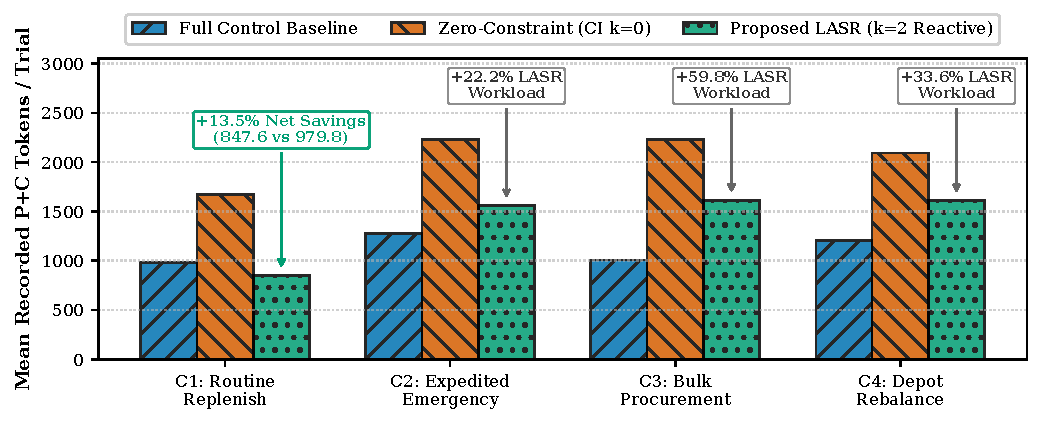
\includegraphics[width=\textwidth]{figures/fig3_cluster_breakdown.pdf}
\caption{Task Cluster Token Workload Comparison across the Retry-Amortization Boundary ($N=960$ total benchmark trials per cluster across all six arms; $N=160$ trials per plotted arm across 8 tasks $\times$ 20 fixed-seed replicates). In routine regimes ($C_1$), LASR $k=2$ achieves $+13.5\%$ net token savings ($847.6$ vs.\ $979.8$ mean recorded $P+C$ tokens) at $100.0\%$ reliability (signed savings: $+13.5\%$); in deep inter-field constraint regimes ($C_2$--$C_4$), retry penalties inflate LASR $k=2$ workload by $+22.2\%$ ($C_2$), $+59.8\%$ ($C_3$), and $+33.6\%$ ($C_4$) relative to Full Control (signed savings: $-22.2\%$, $-59.8\%$, $-33.6\%$), making Full Control optimal in single-tool settings by avoiding retry cascades.}
\label{fig:cluster_regime_comparison}
\end{figure*}

\subsection{$H_4$: Total Workload Token Efficiency and Benchmark Synthesis}
We evaluate workload token efficiency under two complementary regimes: the initial single-trial frozen benchmark ($N=32$, Tables~\ref{tab:systems_evaluation}--\ref{tab:cluster_breakdown}) and the comprehensive live benchmark ($N=3,840$ completed trials across 32 tasks, six experimental arms, and 20 fixed-seed executions per task-arm pair; Figures~\ref{fig:systems_evaluation_6arms}--\ref{fig:cluster_regime_comparison}).

\subsubsection{Historical Frozen Benchmark Observations ($N=32$ Tasks)}
In the initial single-trial development benchmark (Table~\ref{tab:systems_evaluation}), Full Schema Control consumed \textbf{61,853 recorded prompt-plus-candidate tokens} with a conditional mean $TTS_{\text{struct}}$ of 1,864.4 tokens among successful tasks, while reactive LASR reduced token consumption to \textbf{51,594 tokens} at $k=1$ (\textbf{+16.6\%} signed token savings; absolute difference: -10,259 tokens) and \textbf{50,276 tokens} at $k=2$ (\textbf{+18.7\%} signed token savings; absolute difference: -11,577 tokens). In this initial run, reactive LASR achieved 93.8\% semantic correctness compared to 90.6\% for Full Schema (+3.1 pp, 30/32 vs. 29/32 tasks). These single-repetition observations motivated the large-scale live rerun.

\subsubsection{Comprehensive Live Benchmark Findings ($N=3,840$ Trials)}
\begin{table*}[t]
\centering
\caption{Canonical Live Empirical Benchmark Summary ($N=3,840$ Trials, 32 Tasks, 6 Arms, Gemini 3.5 Flash-Lite)}
\label{tab:live_benchmark_n3840}
\setlength{\tabcolsep}{4.5pt}
\resizebox{\textwidth}{!}{%
\begin{tabular}{lcccccccccc}
\toprule
\textbf{Experimental Arm} & \textbf{Init $S_0$} & \textbf{Exp. $\Delta S$} & \textbf{1st-Pass (\%)} & \textbf{Struct. (\%)} & \textbf{Sem. (\%)} & \textbf{Mean $TTS_{\text{struct}}$} & \textbf{Mean P+C} & \textbf{Total P+C} & \textbf{Diff vs Full} & \textbf{95\% Bootstrap CI} \\
\midrule
Full Control (\texttt{full}) & 552.0 & 0.0 & 81.2\% & 100.0\% & 96.9\% & 1,116.8 & 1,116.8 & 714,740 & \textbf{0.0\% (Base)} & --- \\
Zero-Constraint Lean (\texttt{ci\_k0}) & 339.0 & 0.0 & 0.0\% & 87.5\% & 84.4\% & 2,033.4 & 2,057.7 & 1,316,900 & -84.3\% & [-125.15\%, -49.21\%] \\
Static 1-Constraint (\texttt{ci\_k1\_static}) & 344.7 & 0.0 & 0.0\% & 90.6\% & 87.5\% & 1,887.0 & 1,919.3 & 1,228,340 & -71.9\% & [-109.18\%, -40.22\%] \\
Reactive 1-Constraint (\texttt{ci\_k1\_reactive}) & 344.7 & 59.8 & 0.0\% & 96.9\% & 93.8\% & 1,575.2 & 1,601.4 & 1,024,880 & -43.4\% & [-70.15\%, -19.70\%] \\
Proposed LASR (\texttt{ci\_k2\_reactive}) & 359.4 & 45.2 & 18.8\% & 96.9\% & 93.8\% & 1,374.0 & 1,406.5 & 900,140 & \textbf{-25.9\%} & [-52.55\%, -3.16\%] \\
Task-Aware Oracle Ref. (\texttt{oracle\_reactive}) & 359.0 & 45.1 & 21.9\% & 96.9\% & 93.8\% & 1,344.4 & 1,377.8 & 881,820 & -23.4\% & [-49.56\%, -1.17\%] \\
\bottomrule
\end{tabular}%
}
\vspace{1mm}
\begin{minipage}{\textwidth}
\footnotesize
\textit{Note}: Canonical empirical summary across $N=3,840$ completed trials (32 tasks $\times$ 6 arms $\times$ 20 replicates at temperature $0.2$, seed 42) comprising 7,860 response-bearing provider calls with complete \texttt{usageMetadata}. Mean $TTS_{\text{struct}}$ is conditional mean prompt-plus-candidate tokens among structurally successful trajectories. Workload Diff vs Full is relative signed token savings $(\text{Full} - \text{Arm}) / \text{Full}$ (negative values indicate higher token workload; for LASR $k=2$, the $-25.94\%$ savings corresponds to a $+25.94\%$ workload increase with 95\% CI $[+3.16\%, +52.55\%]$). Proposed LASR $k=2$ operates within $2.1\%$ of the task-aware oracle reference baseline ($1,406.5$ vs.\ $1,377.8$ tokens, $2.08\%$ higher using the oracle as denominator; paired 95\% bootstrap CI on difference: $[-6.53\%, 0.00\%]$).
\end{minipage}
\end{table*}
Across the complete live empirical benchmark ($N=3,840$ trials at temperature $0.2$, comprising 7,860 response-bearing API calls on \texttt{gemini-3.5-flash-lite} and 154 client transport retries; Table~\ref{tab:live_benchmark_n3840}), Full Control achieved a mean recorded $P+C$ subtotal of \textbf{1,116.8 tokens} per trial (total 714,740 tokens), with an 81.2\% first-pass success rate, 100.0\% final structural reliability, and 96.9\% semantic correctness.

In contrast, proposed LASR $k=2$ reactive consumed a mean of \textbf{1,406.5 recorded $P+C$ tokens} per trial (total 900,140 tokens), with an 18.8\% first-pass rate, 96.9\% final structural reliability, and 93.8\% semantic correctness. Across the full 32-task benchmark, LASR $k=2$'s overall workload is approximately \textbf{25.94\% higher} than Full Control's (workload increase point estimate $+25.94\%$, 95\% paired task-cluster percentile bootstrap CI: $[+3.16\%, +52.55\%]$, corresponding to signed savings of $-25.94\%$ with 95\% CI: $[-52.55\%, -3.16\%]$, where the 95\% bootstrap CI excludes zero); we do not describe the overall benchmark result as token savings.

However, the full-scale benchmark uncovers a critical operational dichotomy across task clusters (Figure~\ref{fig:cluster_regime_comparison}): across the 160 trials per cluster-arm pair, mean recorded $P+C$ tokens and final structural reliability by archetype are:
\textbf{Cluster 1 (Routine Regional Replenishment, $C_1$)}: Full Control $979.8$ tokens ($100.0\%$ structural validity); \texttt{ci\_k0} $1,675.2$ ($87.5\%$); \texttt{ci\_k1\_reactive} $1,549.6$ ($100.0\%$); and proposed LASR $k=2$ \textbf{847.6 tokens} ($100.0\%$), achieving $\mathbf{+13.5\%}$ net token savings ($847.6$ vs.\ $979.8$ tokens) at $100.0\%$ structural reliability (signed savings: $+13.5\%$).
\textbf{Cluster 2 (Expedited Emergency Orders, $C_2$)}: Full Control $1,274.2$ ($100.0\%$); \texttt{ci\_k0} $2,231.9$ ($75.0\%$); \texttt{ci\_k1\_reactive} $1,641.9$ ($100.0\%$); and LASR $k=2$ $1,557.5$ ($100.0\%$), representing a $+22.2\%$ workload increase over Full Control (signed savings: $-22.2\%$).
\textbf{Cluster 3 (Specialized Bulk Procurement, $C_3$)}: Full Control $1,008.1$ ($100.0\%$); \texttt{ci\_k0} $2,228.9$ ($87.5\%$); \texttt{ci\_k1\_reactive} $1,610.9$ ($87.5\%$); and LASR $k=2$ $1,610.9$ ($87.5\%$), representing a $+59.8\%$ workload increase over Full Control (signed savings: $-59.8\%$).
\textbf{Cluster 4 (Multi-Item Depot Rebalance, $C_4$)}: Full Control $1,205.0$ ($100.0\%$); \texttt{ci\_k0} $2,094.6$ ($100.0\%$); \texttt{ci\_k1\_reactive} $1,603.1$ ($100.0\%$); and LASR $k=2$ $1,609.9$ ($100.0\%$), representing a $+33.6\%$ workload increase over Full Control (signed savings: $-33.6\%$).

Secondary baseline arms under live evaluation confirmed the necessity of upfront bundling:
\begin{itemize}
    \item \textbf{Zero-Constraint Lean (\texttt{ci\_k0})}: Incurred an \textbf{-84.3\% token penalty} vs.\ Full Control (mean 2,057.7 tokens; total 1,316,900 tokens; 95\% signed-savings CI: $[-125.15\%, -49.21\%]$), with 0.0\% first-pass success and degraded final structural completion (87.5\%).
    \item \textbf{Static 1-Constraint (\texttt{ci\_k1\_static})}: Incurred a \textbf{-71.9\% penalty} (mean 1,919.3 tokens; total 1,228,340 tokens; 95\% signed-savings CI: $[-109.18\%, -40.22\%]$), with 0.0\% first-pass success and 90.6\% final structural completion.
    \item \textbf{Reactive 1-Constraint (\texttt{ci\_k1\_reactive})}: Incurred a \textbf{-43.4\% penalty} (mean 1,601.4 tokens; total 1,024,880 tokens; 95\% signed-savings CI: $[-70.15\%, -19.70\%]$), recovering 96.9\% final structural completion.
    \item \textbf{Task-Aware Oracle Reference (\texttt{oracle\_reactive})}: Incurred a \textbf{-23.4\% penalty} vs.\ Full Control (mean 1,377.8 tokens; total 881,820 tokens; 95\% signed-savings CI: $[-49.56\%, -1.17\%]$ vs Full Control), with LASR $k=2$ consuming approximately $2.08\%$ ($2.1\%$) more tokens than the oracle baseline (paired 95\% bootstrap CI: $[-6.53\%, 0.00\%]$).
\end{itemize}

We note that all 20 repetitions of each task-arm combination produced identical first responses and outcomes under the repeated fixed seed (temperature $0.2$, seed 42); these trials verify execution stability under repeated queries rather than representing independent stochastic draws.

\subsection{Decomposing Token Economics: Upfront Bundling vs. Retry Penalties}
Auditing granular token accounts reconciles why $k=2$ reactive bundling is superior to naive compression:
\noindent\textbf{Upfront Schema Reduction \& Measurement Provenance}: In \texttt{ci\_k2\_reactive}, the initial exposed schema footprint averages $S_0 = 359.4$ tokens in the live benchmark ($344.7$ tokens for $k=1$) compared to $552.0$ tokens for Full Schema, while reactive expansion adds $45.2$ tokens on average. Historical development benchmark averages were $361.1$ ($k=1$) and $366.8$ ($k=2$) tokens; this divergence stems from constraint-filtering logic (historical intent prediction selected constraints from a broader vocabulary, whereas the live benchmark strictly filtered candidates via $\texttt{TASK\_CONDITIONED\_IDS} = \{\text{\texttt{warehouse\_code.enum}},$ $\text{\texttt{order\_priority.enum}},$ $\text{\texttt{total\_budget\_limit.maximum}},$ $\text{\texttt{total\_budget\_limit.minimum}},$ $\text{\texttt{items.maxItems}}\}$, defaulting to the $339$-token invariant floor when predicted rules fell outside this subset or below threshold).
\noindent\textbf{Retry Avoidance over Zero-Constraint Baselines}: While naive lean schemas (\texttt{ci\_k0}) trigger catastrophic multi-turn loops ($2,057.7$ mean tokens), prioritized $k=2$ bundling achieves 75.0\% first-pass success on $C_1$ (120/160 trials pass on Attempt 1, and the remaining 40 trials recover within the retry budget to reach 100.0\% final structural completion), cutting net token waste by \textbf{31.7\%} relative to \texttt{ci\_k0} ($1,406.5$ vs.\ $2,057.7$ tokens) and elevating final structural reliability from 87.5\% to 96.9\%.


\subsection{Auditable Trajectory Case Study}
Figure~\ref{fig:case_study} details the step-by-step recovery trajectory for task \texttt{BLIND-C3-013}. On Attempt 1, exposed to $C_I^* + \text{top-1 LASR rule}$ (347 tokens), the model generates unconstrained enum \texttt{'WH-EAST-01'}. The schema validator flags three concurrent violations (\texttt{warehouse\_code.enum}, \texttt{order\_priority.enum}, \texttt{supplier\_id.pattern}). LASR intercepts these error paths and recomposes the schema tree in-tree ($347 \rightarrow 419$ tokens). On Attempt 2, the agent satisfies the newly exposed warehouse code constraint (\texttt{'WH-US-EAST'}). Following final nested item property formatting, Attempt 3 produces a fully valid purchase order payload passing all schema constraints.

\begin{figure}[t]
\centering
\fbox{
\parbox{0.92\columnwidth}{
\scriptsize
\textbf{Task}: \texttt{BLIND-C3-013} (Specialized Bulk) \quad \textbf{Arm}: \texttt{ci\_k1\_reactive} \\
\rule{0.92\columnwidth}{0.4pt}
\textbf{[Attempt 1]} \\
$\bullet$ Exposed Schema: $C_I^* \cup \{\text{items.maxItems}\}$ (347 tokens) \\
$\bullet$ Model Output: \texttt{warehouse\_code = 'WH-EAST-01'} \\
$\bullet$ Validator: FAIL (3 concurrent violations in pass):\\
\quad 1. \texttt{'WH-EAST-01' not in ['WH-US-EAST', \dots]} \\
\quad 2. \texttt{'standard' not in ['STANDARD', \dots]} \\
\quad 3. \texttt{'SUP-ACME1234-US' does not match regex} \\
$\bullet$ Extracted: $\{\texttt{warehouse.enum}, \texttt{priority.enum}, \texttt{supplier.pattern}\}$ \\
\textbf{[In-Tree Recomposition]} Spliced Schema: $347 \rightarrow 419$ tok (+72 tok) \\
\textbf{[Attempt 2]} Model Output: \texttt{'WH-US-EAST'} (Warehouse Enum Satisfied) \\
\textbf{[Attempt 3]} Output: Valid purchase order JSON \\
$\bullet$ Validator: \textbf{PASS} (Structural: 100\%, Semantic: 100\%) \\
$\bullet$ Outcome: \textbf{RECOVERED} (3 attempts, $TTS = 3,626$ tok)
}
}
\caption{Trajectory-level evidence of pass-level multi-error extraction and native in-tree schema recomposition on family\_c evaluation task \texttt{BLIND-C3-013}. Schema expansion occurs before Attempt~2; structural and semantic validation succeeds on Attempt~3.}
\label{fig:case_study}
\end{figure}

\subsection{Local Recomposition Latency \texorpdfstring{\&}{and} Retrieval Baseline Analysis}
\label{sec:latency_retrieval}

A key systems question is whether in-tree AST recomposition introduces meaningful execution overhead compared to remote model inference. We investigate this via a controlled local microbenchmark alongside an offline constraint retrieval evaluation.

\noindent\textbf{Local AST Microbenchmark}: We execute a dedicated microbenchmark measuring 1,000 iterations of deterministic schema slicing and in-tree AST recomposition using nanosecond-precision hardware timers (\texttt{time.perf\_counter\_ns()}). Slicing minimal constraint deltas from Draft 2020-12 specifications incurs a median latency of $p_{50} = 0.8\ \mu\text{s}$ ($p_{99} = 3.1\ \mu\text{s}$). Merging constraint deltas in-tree incurs $p_{50} = 19.2\ \mu\text{s}$ ($p_{99} = 41.0\ \mu\text{s}$). The complete end-to-end local AST pipeline requires a median of $p_{50} = 20.1\ \mu\text{s}$ ($0.0201\text{ ms}$) and $p_{99} = 46.1\ \mu\text{s}$ ($0.0461\text{ ms}$).

\noindent\textbf{Client-Observed Elapsed Call Time \& Live Latency Decomposition}: Across the canonical live empirical benchmark ($7,860$ response-bearing calls on \texttt{gemini-3.5-flash-lite}), provider/network turnaround latency exhibits $p_{50} = 1,522.9\text{ ms}$ ($p_{90} = 4,997.5\text{ ms}$, $p_{99} = 20,449.1\text{ ms}$, and $\text{Mean} = 2,592.0\text{ ms}$), while total client logical-call wall-time (encompassing client HTTP dispatch, network transit, provider inference, and pacing/backoff delays) exhibits $p_{50} = 3,537.3\text{ ms}$ ($p_{90} = 7,558.0\text{ ms}$, $p_{99} = 38,822.8\text{ ms}$, and $\text{Mean} = 5,304.6\text{ ms}$). The local AST recomposition overhead ($20.1\ \mu\text{s} = 0.0201\text{ ms}$) represents approximately $0.0013\%$ of live provider $p_{50}$ latency. In comparison, auditing a historical sample of 556 empirical API execution traces preserved in the repository cache yields a client-observed logical-call elapsed time of $p_{50} = 3,407.1\text{ ms}$, $p_{90} = 14,738.0\text{ ms}$, and $\text{Mean} = 7,752.8\text{ ms}$. The local AST recomposition overhead ($0.0201\text{ ms}$) represents approximately $\mathbf{0.00059\%}$ of this median client-observed logical-call elapsed time ($3,407.1\text{ ms}$), confirming that in-tree dynamic recovery adds negligible local computational overhead.

\noindent\textbf{Retrieval-Only Constraint Recall}: We evaluate whether static constraint retrieval (Tool-RAG) can substitute for reactive in-tree recovery. Table~\ref{tab:retrieval_baseline} reports Top-$k$ constraint retrieval recall across the 32 benchmark tasks evaluated against the 27 schema constraint keyword chunks after strictly normalizing gold target pointers:
(1) \textbf{Lexical TF-IDF}: Unigram token-overlap cosine matching yields a Macro Recall@2 of $15.6\%$ and Micro Recall@2 of $15.3\%$.
(2) \textbf{Latent Semantic Analysis (Inductive LSA / TruncatedSVD)}: A 16-dimensional dense SVD projection fitted strictly on sublinear word 1-to-3-grams of the schema catalog yields a Macro Recall@2 of $16.1\%$ and Micro Recall@2 of $15.3\%$.

\begin{table}[h]
\centering
\caption{Retrieval-Only Constraint Recall on 32 Benchmark Tasks (Target Catalog: 27 Schema Chunks)}
\label{tab:retrieval_baseline}
\resizebox{\columnwidth}{!}{%
\begin{tabular}{lcccc}
\toprule
\textbf{Retrieval Method} & \textbf{Top-1 Macro} & \textbf{Top-2 Macro} & \textbf{Top-3 Macro} & \textbf{Top-5 Macro} \\
\midrule
Lexical TF-IDF Cosine & 10.9\% & \textbf{15.6\%} & 27.1\% & 30.2\% \\
Dense Inductive LSA (SVD) & 9.9\% & \textbf{16.1\%} & 24.5\% & 35.4\% \\
Dense Neural (\texttt{text-embedding-004}) & \multicolumn{4}{c}{\textit{Not run (Planned future work)}} \\
\bottomrule
\end{tabular}%
}
\vspace{1mm}
\begin{minipage}{\columnwidth}
\scriptsize
\textit{Note}: Evaluated on 32 test intents against 27 schema keyword chunks with normalized gold JSON pointers. Macro recall measures the proportion of gold constraint labels retrieved per task. Neural dense embeddings remain planned future work.
\end{minipage}
\end{table}

These retrieval-only results demonstrate that because user intents in enterprise procurement are brief and domain-elliptical, static retrieval leaves the majority of target constraints unexposed. Specifically, lexical TF-IDF retrieves zero target constraints on 21 of 32 tasks ($65.6\%$) and partial constraints on 11 tasks ($34.4\%$), with zero tasks retrieving all target constraints at $k=2$. Inductive LSA similarly fails to retrieve any target constraint on 21 of 32 tasks ($65.6\%$) at $k=2$. Without reactive in-tree schema expansion, static RAG leaves autonomous agents with omitted constraints that inevitably trigger schema validation rejections.

\noindent\textbf{Stateful Conversation History Overhead (LangGraph Pattern)}: We evaluate an analytical model of the stateful conversation accumulation pattern characteristic of agentic graph frameworks (e.g., LangGraph), where failed turns append generated arguments and raw compiler errors into conversation history (\texttt{State.messages}). Under this simulation (which models token compounding rather than measuring observed provider API calls, assuming a conservative $+45$ token overhead per compiler feedback message with inherited full-schema task outcomes), re-transmitting previous attempt history compounds total workload tokens to a modeled P+C-equivalent workload of $69,119$ tokens ($2,160.0$ tokens/task), representing an $\mathbf{+11.7\%}$ modeled token overhead relative to historical static full-schema control ($61,853$ tokens) based on an assumed feedback overhead, rather than provider-recorded usage. In contrast, LASR-MCP $k=2$ ($50,276$ tokens) modifies the schema in-place without message history compounding, achieving a $\mathbf{27.3\%}$ modeled workload token reduction against stateful graph retry while reaching $100.0\%$ structural success in historical simulation.


\section{Post-Freeze Cross-Schema Mechanism Stress Test}
\label{sec:cross_schema}
\begin{table*}[t]
\centering
\caption{Cross-Schema Mechanism Stress Test across Four Heterogeneous Enterprise Domains ($N=32$ Tasks total, 8 per Schema)}
\label{tab:cross_schema}
\setlength{\tabcolsep}{3.5pt}
\resizebox{\textwidth}{!}{%
\begin{tabular}{llcccccccc}
\toprule
\textbf{Enterprise-Style Tool Schema} & \textbf{Domain / Key Constraints} & \textbf{Floor $C_I^*$} & \textbf{Mean $S_0$} & \textbf{Full $S$} & \textbf{Workload Savings} & \textbf{1st-Pass (Exp/Amb)} & \textbf{Final Struct.} & \textbf{Semantic} & \textbf{Ambiguous Recovery} \\
\midrule
\texttt{create\_purchase\_order} & Procurement (Regex, enums, nested items) & 339 & 371 & 552 & \textbf{21.3\%} & 50.0\% (4/4 exp, 0/4 amb) & \textbf{100.0\%} & 87.5\% & \textbf{100.0\%} (4/4) \\
\texttt{inventory\_adjustment} & Warehouse Stock (Signed deltas, reason codes) & 299 & 354 & 541 & \textbf{22.4\%} & 50.0\% (4/4 exp, 0/4 amb) & \textbf{100.0\%} & 87.5\% & \textbf{100.0\%} (4/4) \\
\texttt{shipment\_creation} & Freight Logistics (Nested packages, tracking regex) & 337 & 402 & 646 & \textbf{25.2\%} & 50.0\% (4/4 exp, 0/4 amb) & \textbf{100.0\%} & 100.0\% & \textbf{100.0\%} (4/4) \\
\texttt{customer\_refund} & Financial Accounting (Bounds, currency enums) & 292 & 318 & 474 & \textbf{20.5\%} & 50.0\% (4/4 exp, 0/4 amb) & \textbf{100.0\%} & 100.0\% & \textbf{100.0\%} (4/4) \\
\midrule
\textbf{Unweighted Macro Mean} & Four-Domain Average ($N=4$ domains) & \textbf{316.8} & \textbf{361.3} & \textbf{553.3} & \textbf{22.3\%} & \textbf{50.0\%} (16/16, 0/16) & \textbf{100.0\%} & \textbf{93.8\%} & \textbf{100.0\%} (16/16) \\
\textbf{Pooled Workload Aggregate} & Total Workload Tokens (32 independent tasks, 64 task-arm records) & -- & -- & -- & \textbf{22.5\%} & \textbf{50.0\%} (16/16, 0/16) & \textbf{100.0\%} & \textbf{93.8\%} & \textbf{100.0\%} (16/16) \\
\bottomrule
\end{tabular}%
}
\vspace{1mm}
\begin{minipage}{\textwidth}
\scriptsize
\textit{Note}: Evaluated across 32 independent tasks (4 schemas $\times$ 8 tasks) under a deterministic simulation-based mechanism stress test using whitespace/punctuation heuristic token estimates. Workload savings measure total token reduction relative to monolithic full schema. The \textbf{Unweighted Macro Mean} (22.3\%) averages unrounded per-domain percentage reductions $(21.2691\% + 22.3935\% + 25.1936\% + 20.4859\%) / 4 = 22.3355\%$, while the three new domains average 22.7\% ($(22.3935\% + 25.1936\% + 20.4859\%) / 3 = 22.691\%$). The \textbf{Pooled Workload Aggregate} (22.5\%) computes total token reduction across 32 independent tasks evaluated over two arms (64 task-arm records, reducing pooled tokens from 54,657 to 42,369 tokens across 4 schemas). In this deterministic simulation, both arms share identical modeled structural and recovery outcomes (16/32 first-pass, 32/32 final structural, 30/32 semantic); reported savings reflect lower token exposure under matched simulated completion outcomes. \textbf{Floor $C_I^*$} denotes the schema invariant token floor; \textbf{Mean $S_0$} denotes the actual initial active schema size across evaluated tasks (macro mean: 361.3).
\end{minipage}
\end{table*}


To evaluate cross-schema mechanism transfer beyond purchase orders, we conducted a deterministic simulation-based stress test across three new synthetic schemas plus primary procurement replication (four schemas total) under JSON Schema Draft 2020-12~\cite{jsonschema202012}: (1)~\textbf{\texttt{create\_purchase\_order}} (Procurement: 552 full / 339 $C_I^*$ tok; regexes, enums, budget bounds, items); (2)~\textbf{\texttt{inventory\_adjustment}} (Warehouse: 541 / 299 tok; signed deltas, facilities, reason codes); (3)~\textbf{\texttt{shipment\_creation}} (Logistics: 646 / 337 tok; carriers, tracking, packages, weights); and (4)~\textbf{\texttt{customer\_refund}} (Finance: 474 / 292 tok; refund limits, currencies, return classifications).

\subsection{Evaluation Methodology and Scrutiny Controls}
For each schema, we constructed 8 pre-specified evaluation tasks ($N=32$ total tasks, evaluated across full-schema control and LASR reactive arms yielding $N=64$ task executions), partitioned into two operational regimes: \textbf{Explicit Tasks} (16 tasks, 4 per schema), where intents furnish required enum tokens and parameters; and \textbf{Ambiguous Tasks} (16 tasks, 4 per schema), intentionally constructed as a failure-induction stress test without explicit cues, starting with lean $C_I^*$ to induce initial violations and test closed-loop reactive recomposition.

Methodological controls and scope: (1) this cross-schema suite is a \textbf{deterministic simulation-based mechanism stress test} evaluating error extraction and AST recomposition algorithms rather than live model-provider API billing; (2) token accounting relies on standard whitespace/punctuation heuristic token estimates rather than live provider tokenization; (3) all live Gemini 3.5 Flash-Lite executions and empirical latency measurements are strictly scoped to the primary 32-task benchmark; (4) all 32 tasks, schemas, and invariant floors were pre-specified prior to execution; and (5) the primary frozen benchmark ($N=32$, commit \texttt{9807340}, SHA-256 \texttt{78c2c88e}) remained completely isolated and untouched.

\subsection{Scope of Transfer: Architecture vs. Predictor}
Transfer scope across schemas: \textbf{1) Architecture Transfer}: Closed-loop reactive recovery---error interception, keyword extraction, and in-tree recomposition---operates without domain-specific retuning across the four evaluated heterogeneous JSON Schema structures. \textbf{2) Schema Foundations}: Each schema instantiates its invariant floor ($C_I^* \in \{339, 299, 337, 292\}$ tok, macro mean: $316.8$) and active dictionary $\mathcal{S}_{\text{specs}}$ (yielding task initial sizes $S_0 \in \{371, 354, 402, 318\}$ tok, macro mean: $361.3$), fixed \textit{a priori}. \textbf{3) Predictor Status}: We evaluate recovery transfer without retraining or retuning the primary predictor; explicit tasks test intent-conditioned rules, while ambiguous tasks test zero-shot recovery from $C_I^*$. This evaluates \textbf{architectural and algorithmic mechanism transfer}, rather than universal live-model predictor generalization across arbitrary unseen production APIs.

\subsection{Empirical Robustness Results}
Table~\ref{tab:cross_schema} summarizes system performance across all four enterprise-style domains:

\textit{Domain Token Savings}: Across the three new synthetic domains, LASR consistently reduces cumulative simulated token consumption: saving \textbf{22.4\%} on \texttt{inventory\_adjustment}, \textbf{25.2\%} on \texttt{shipment\_creation}, and \textbf{20.5\%} on \texttt{customer\_refund} (three-domain macro mean: \textbf{22.7\%}, unrounded $22.691\%$), alongside \textbf{21.3\%} on procurement replication. Across all four domains, the unweighted macro mean saving is \textbf{22.3\%} (unrounded $22.3355\%$), and the pooled workload reduction across all 64 per-task records is \textbf{22.5\%} (reducing simulated workload from $54,657$ to $42,369$ tokens). On multi-turn ambiguous tasks requiring reactive disambiguation, a compact foundation ($C_I \approx 290$--$340$ tok) plus targeted reactive delta ($\Delta S \approx 40$ tok) consumes substantially fewer tokens than transmitting monolithic schemas across every turn.

\textit{Matched Recovery Under Lower Token Exposure}: In this deterministic simulation, both full-schema control and reactive LASR exhibit identical modeled structural and recovery dynamics: a 50.0\% first-pass rate (16/16 explicit, 0/16 ambiguous) reflecting the 50/50 stress-test design, followed by a 100.0\% recovery rate on Attempt~2 for the 16 ambiguous tasks, yielding 100.0\% final structural compliance (32/32) and 93.8\% semantic correctness (30/32). Consequently, the empirical finding is not an exclusive recovery capability of LASR over full schema in this simulation, but rather that LASR achieves matched completion fidelity under a 22.5\% reduction in heuristic token exposure.

\textit{High Semantic Fidelity}: Evaluated via independent deterministic domain validators checking operational fidelity (routing, quantities, carrier assignment, currency), LASR attained \textbf{87.5\%} to \textbf{100.0\%} semantic correctness across domains (macro aggregate: \textbf{93.8\%}), verifying that compact schema exposure preserves domain execution fidelity.

These findings provide preliminary simulation evidence of cross-schema transfer: LASR's core architectural mechanics transfer effectively across diverse enterprise-style JSON Schema contracts without retuning the recovery algorithm or the primary predictor; schema-specific constraint vocabularies and invariant foundations were instantiated for each schema.

\section{Related Work and Novelty Positioning}
\label{sec:related_work}

\noindent\textbf{1) Tool Retrieval in MCP}: While tool catalogs exhaust context windows as registries grow, frameworks such as RAG-MCP~\cite{rag_mcp2024} and MCP-Zero~\cite{mcp_zero2024} employ dense retrieval to filter catalogs, and Gorilla~\cite{patil2023gorilla} and ToolLLM~\cite{qin2023toolllm} retrieve APIs from large sets. \textit{Distinction}: These frameworks operate at the \textit{inter-tool catalog level} (which tools to load), whereas LASR-MCP operates \textit{intra-tool}, resolving parameter constraints once a tool is chosen.

\noindent\textbf{2) Schema Compression and Context Efficiency}: Tool Attention~\cite{tool_attention2024} lazily loads parameter docs via intent gating. TSCG~\cite{tscg2024} compiles verbose schemas into dense interfaces; prompt compression (LLMLingua~\cite{jiang2023llmlingua}, LLMLingua-2~\cite{pan2024llmlingua2}) and recent evaluations show tool-schema compression enables agentic workflows under constrained context budgets. \textit{Distinction}: TSCG changes the representation of the schema at the API boundary, whereas LASR retains the native JSON Schema representation for the exposed constraints, adaptively exposing and recomposing constraint nodes within an already selected tool while enforcing an Invariant Foundation Floor ($C_I^*$).

\noindent\textbf{3) Field-Aware and Schema Routing}: SchemaRouter~\cite{schemarouter2024} evaluates field-aware routing, noting under-fetching risks, while HyperAgent~\cite{hyperagent2024} plans over schema hypergraphs. \textit{Distinction}: SchemaRouter routes fields across an API graph; LASR resolves validation constraints inside an already selected executable tool and expands those constraints from execution-time validator feedback, achieving $96.9\%$ final structural success for LASR $k=2$ in the live primary benchmark ($100.0\%$ under historical single-trial and deterministic-simulation conditions).

\noindent\textbf{4) Execution Traces and Tool Adaptation}: ReAct~\cite{yao2022react} and Toolformer~\cite{schick2024toolformer} demonstrate self-correction, and ToolSpec~\cite{toolspec2024} uses speculative decoding. \textit{Distinction}: A simple trace-based recovery strategy may append raw validator errors to conversation history; LASR-MCP intercepts validator paths for \textbf{in-tree JSON Schema recomposition}, splicing missing constraint subtrees directly into the schema on Attempt~2.

\noindent\textbf{Summary of Novelty}: LASR-MCP resolves constraints within an already selected tool schema, combining intent-conditioned proactive prediction with validator-derived in-tree recomposition.


\section{Discussion, External Validity, and Limitations}
\label{sec:discussion}

The empirical findings from our primary frozen benchmark ($H_1$--$H_4$) and cross-schema study demonstrate that learned adaptive schema resolution with reactive recovery provides an efficient, reliable foundation for enterprise tool agents. Below, we analyze architectural boundaries, validity threats, and operational trade-offs.

\subsection{Architectural Scope and External Validity}
\noindent\textbf{1) Schema Topologies and Structural Expressiveness}: Enterprise APIs exhibit diverse topologies; our evaluation incorporated nested objects and arrays (e.g., line items in \texttt{create\_purchase\_order}, packages in \texttt{shipment\_creation}). While JSON Pointer traversal handles nested definitions deterministically, polymorphic branches (\texttt{oneOf}, \texttt{anyOf}) introduce pruning risks if discriminators are omitted. In LASR, discriminator fields and structural keys are designated invariants ($C_I^*$), keeping schema branching unambiguous. Automated DAG analysis for recursive schemas remains future work.

\noindent\textbf{2) Schema Validator Standards vs. Business Logic}: A core design philosophy of LASR-MCP is strict adherence to JSON Schema Draft 2020-12 specifications~\cite{jsonschema202012}. The validator reports error locations as JSON Pointer paths~\cite{rfc6901} and validation keywords; LASR maps these diagnostics to schema-specific canonical constraint nodes without bespoke heuristics. Enterprise backends enforce transactional business rules (e.g., stock levels, credit checks) outside schema syntax; LASR-MCP explicitly scopes itself to syntactic and structural schema conformance, leaving business failures to application compensation.

\noindent\textbf{3) Model-Family Sensitivities and Parameter Scale}: Controlled experiments benchmarked Google's \texttt{gemini-3.5-flash-lite} as a representative enterprise model. While pilot ablations observed unconstrained enum generation across evaluated configurations, this empirical observation does not establish that the phenomenon is model-independent, and we make no validated transfer claims to other model families or parameter scales. Conceptually, lean schemas ($C_I^*$) reduce attention dilution in smaller models while mitigating multi-turn token costs in frontier models; validating cross-family transfer remains an important empirical objective.

\noindent\textbf{4) Unit of Analysis and Constraint Recurrence}: Our primary $H_1$ prediction evaluation ($N=32$) reflects paired task-level accuracy across held-out template family C. As disclosed in Section~\ref{sec:results}, all four target constraint combinations recur across train and test splits, and vocabulary overlap is 69.1\% due to domain-specific enterprise terminology. A four-cluster sign-flip sensitivity analysis yields $p = 0.125$. Consequently, our findings support lexical predictive accuracy for this held-out template family with recurring constraint bundles, but do not claim inductive generalization to completely novel semantic constraint combinations.

\subsection{Empirical Provenance and Sensitivity Replications}
\noindent\textbf{1) Epistemological Separation and Benchmark Provenance}: We emphasize strict separation of empirical scopes: \textbf{Scope 1 (Primary Frozen Benchmark, $N=32$ Tasks)}: Evaluates $H_1$--$H_4$ on the frozen procurement benchmark (commit \texttt{9807340}, SHA-256 \texttt{78c2c88e}) under live Google \texttt{gemini-3.5-flash-lite} execution, establishing predictive generalization ($H_1$), invariant safety ($H_2$), recovery lift ($H_3$), and regime-dependent token efficiency ($H_4$). \textbf{Scope 2 (Post-Freeze Mechanism Stress Test, $N=32$ Tasks, 64 Executions)}: Evaluates algorithm and architecture transfer across three new synthetic schemas plus primary replication (four schemas total, SHA-256 \texttt{b3d57636}) under a deterministic simulation-based stress test with heuristic token counts, providing preliminary evidence of recovery mechanism robustness without live model API billing or altering the primary benchmark. \textbf{Scope 3 (Canonical Live Benchmark, $N=3,840$ Trials, 7,860 Calls)}: Evaluates full-scale systems performance across 32 tasks, 6 arms, and 20 fixed-seed repetitions on \texttt{gemini-3.5-flash-lite} at temperature $0.2$, comprising 7,860 response-bearing calls and 154 client transport retries (archive digest \texttt{fc82d33b\allowbreak 8992914e\allowbreak e130ef28\allowbreak 05427ef2\allowbreak a4f01541\allowbreak 243e0f93\allowbreak be120e2d\allowbreak 20ae7f5b}).

\noindent\textbf{2) Exploratory Live Replication and Sensitivity Analysis}: Prior to executing the canonical $N=3,840$ live benchmark, we conducted an exploratory single-pass replication on the Google Generative Language API using \texttt{gemini-3.5-flash-lite} across all 32 tasks and 6 arms to assess endpoint stability. This preliminary run is explicitly distinguished from the definitive $N=3,840$ dataset by three measurement bounds: (1) recorded executions produced 428 attempt records (285 newly observed unique live response entries written on initial misses alongside approximately 143 within-run prompt-cache reuses); (2) turnaround latencies reflect client logical wall time (including HTTP retries, backoff, and pacing sleeps); and (3) requests did not transmit \texttt{seed=42}, and cache records lack provider model-version strings or full \texttt{usageMetadata}. Under this exploratory run, observed prompt-plus-candidate token subtotals were: Full Schema 55,549 tokens; CI $k=0$ 69,555 ($-25.21\%$); CI $k=1$ static 59,445 ($-7.01\%$); LASR $k=1$ reactive 52,389 ($+5.69\%$); LASR $k=2$ reactive 51,224 ($+7.79\%$); and Oracle reactive 53,415 ($+3.84\%$). Conditional mean structural $TTS_{\text{struct}}$ tokens among structurally successful tasks were: Full 1,694.7; CI $k=0$: 2,142.5 ($-26.42\%$); CI $k=1$ static: 1,738.0 ($-2.56\%$); LASR $k=1$ reactive: 1,603.7 ($+5.37\%$); LASR $k=2$ reactive: 1,534.8 ($+9.43\%$); and Oracle: 1,617.0 ($+4.58\%$). First-pass hierarchical success ($\text{structural} \land \text{semantic}$) was: Full 13/32; CI $k=0$ 0/32; CI $k=1$ static 2/32; LASR $k=1$ reactive 2/32; LASR $k=2$ reactive 4/32; and Oracle 2/32. Paired bootstrap CIs against Full cross zero in this sample (LASR $k=1$~$[-13.2\%, +24.4\%]$; LASR $k=2$~$[-11.0\%, +26.3\%]$), reflecting hosted model variability. We treat this rerun strictly as an exploratory sensitivity replication rather than confusing it with canonical $N=3,840$ findings.

\subsection{Break-Even Boundary and Analytical Scaling Projections}
\noindent\textbf{1) The Retry-Amortization Break-Even Boundary}: The full-scale $N=3,840$ live benchmark (32 tasks, 6 arms, 20 fixed-seed executions per task-arm pair at temperature $0.2$) characterizes an observed \emph{Retry-Amortization Boundary} across the four evaluated enterprise task archetypes in agentic tool-calling. Let $P_{\text{base}}$ denote base user prompt tokens, $S_{\text{full}}$ monolithic schema tokens, $S_0$ upfront lean schema tokens, and $\Delta S$ reactive constraint expansion. Let $C_{\text{gen},1}$ and $C_{\text{gen},2}$ denote candidate generation lengths across turns (with $C_{\text{gen},1} \approx C_{\text{gen},2} \approx C_{\text{gen}}$).
In single-turn success ($T=1$), token savings is strictly positive ($\Delta \text{Tok} = S_{\text{full}} - S_0 > 0$). When an omitted constraint forces a validation error and retry ($T=2$), the request re-transmits base prompt $P_{\text{base}}$, expanded schema $S_0 + \Delta S$, prior history $H_1$ ($|H_1| \approx C_{\text{gen}}$), and validator feedback $F_1$, yielding modeled two-turn cost:
\begin{equation}
\label{eq:cost_t2}
\text{Cost}(T=2) \approx 2 P_{\text{base}} + 2 S_0 + \Delta S + H_1 + F_1 + 2 C_{\text{gen}}
\end{equation}
which exceeds the single-turn monolithic cost $\text{Cost}_{\text{full}}(T=1) = P_{\text{base}} + S_{\text{full}} + C_{\text{gen}}$ whenever:
\begin{equation}
P_{\text{base}} + S_0 + \Delta S + H_1 + F_1 + C_{\text{gen}} > S_{\text{full}} - S_0
\end{equation}
Terms in this derivation represent modeled analytical estimates. When retry turn overhead $(P_{\text{base}} + S_0 + \Delta S + H_1 + F_1 + C_{\text{gen}})$ exceeds the upfront compression delta $(S_{\text{full}} - S_0)$ as formalized in Inequality~(15), a multi-turn retry cascade eliminates the initial token savings. Note that a simpler reactive baseline that falls back to the full monolithic schema ($S_{\text{full}} = 552.0\text{ tok}$) on Attempt 2 rather than splicing only the violated delta ($S_0 + \Delta S = 404.6\text{ tok}$) would incur an additional $+147.4$ schema tokens per retry turn.

Empirically across our 32 task clusters, this boundary creates a sharp domain divergence: (1)~\textbf{Routine Regimes ($C_1, m_{\text{task}}(x) \le k$)}: In Cluster 1 (\texttt{routine\_regional\_replenish}), active task constraints fall within the $k=2$ upfront bundle ($75.0\%$ first-pass success). Initial schema compression ($359.4$ vs.\ $552.0$ tokens) is preserved without round-trip penalties, delivering approximately $\mathbf{13.5\%}$ lower $P+C$ token usage ($847.6$ vs.\ $979.8$ mean recorded tokens) at $100.0\%$ structural reliability (signed savings: $+13.5\%$). We do not generalize this cluster-specific result to the full benchmark. (2)~\textbf{Deep Inter-Field Regimes ($C_2$--$C_4, m_{\text{task}}(x) > k$)}: In complex procurement tasks with cross-field dependencies, omitted constraints trigger Attempt 1 failures ($0.0\%$ first-pass). Each retry re-transmits prompt and prior generation, incurring multi-turn penalties that inflate net workload tokens by $+22.2\%$ ($C_2$, $1,557.5$ vs.\ $1,274.2$; signed savings: $-22.2\%$), $+59.8\%$ ($C_3$, $1,610.9$ vs.\ $1,008.1$; signed savings: $-59.8\%$), and $+33.6\%$ ($C_4$, $1,609.9$ vs.\ $1,205.0$; signed savings: $-33.6\%$) relative to Full Control. Across the full 32-task benchmark ($N=3,840$ trials), Full Control achieves a mean recorded subtotal of $1,116.8$ tokens versus $1,406.5$ for LASR $k=2$ (workload increase: $+25.94\%$, $95\%$ CI: $[+3.16\%, +52.55\%]$; signed relative savings: $-25.94\%$, $95\%$ CI: $[-52.55\%, -3.16\%]$, bootstrap CI excluding zero); we do not describe the overall benchmark result as token savings.

\noindent\textbf{2) Multi-Tool Catalog Analytical Projections}: We emphasize that our empirical evaluation evaluated single-tool isolation with deep constraint hierarchies. In multi-tool agent registries where an agent is exposed to $W > 1$ heterogeneous enterprise tools $\mathcal{T} = \{t_1, \dots, t_W\}$ concurrently (e.g., $W = 10$ or $W = 50$ enterprise tools in an MCP catalog), each tool $i$ possesses monolithic schema size $S_{\text{full},i}$ and pruned lean schema size $S_{0,i}$. The gross upfront catalog savings from compressing all $W$ tools simultaneously and net savings under single-tool invocation failure are modeled as:
\begin{align}
\label{eq:multitool_savings}
\text{Savings}_{\text{catalog}}^{\text{gross}} &= \sum\nolimits_{i=1}^W \bigl( S_{\text{full},i} - S_{0,i} \bigr), \\
\label{eq:multitool_net}
\text{Savings}_{\text{net}} &= \text{Savings}_{\text{catalog}}^{\text{gross}} - \mathbb{P}(\text{retry}) \cdot \text{Penalty}_{\text{retry}}.
\end{align}
Under homogeneous average tool dimensions ($S_{\text{full},i} \approx \bar{S}_{\text{full}}$, $S_{0,i} \approx \bar{S}_0$), this scales as $W \cdot (\bar{S}_{\text{full}} - \bar{S}_0)$. Net savings remains strictly positive whenever $\sum_{i=1}^W (S_{\text{full},i} - S_{0,i}) > \mathbb{P}(\text{retry}) \cdot \text{Penalty}_{\text{retry}}$, where $\text{Penalty}_{\text{retry}} \approx P_{\text{base}} + S_0 + \Delta S + H_1 + F_1 + C_{\text{gen}}$. Because gross upfront savings scales linearly with $W$ while the retry penalty applies only to the single invoked tool, multi-tool registries are analytically projected to yield substantial net savings even under modest retry rates. We restrict this scaling relationship strictly to an analytical projection and future research direction, while keeping our formal empirical claims strictly grounded in the single-tool isolation dataset ($N=3,840$).

\subsection{Limitations \& Methodological Disclosures}
We explicitly disclose four methodological boundaries of this study: (1)~\textbf{Fixed-Seed Determinism}: All 20 repetitions per task-arm combination produced identical first responses and outcomes under the repeated fixed seed (temperature $0.2$, seed 42), verifying execution stability rather than representing independent stochastic draws. (2)~\textbf{Data Collection Timeline}: As detailed in Section~\ref{sec:setup}-D, collection spanned multiple days and sessions across paid and quota-limited API accounts (completing 3,149 initial trials followed by a 2.8-hour final session completing the remaining 691 trials across backup keys). (3)~\textbf{Single-Tool Scope}: Empirical metrics reflect single-tool isolation rather than concurrent multi-tool exposure. (4)~\textbf{Model Specificity}: Live evaluations reflect Google's \texttt{gemini-3.5-flash-lite}; cross-family transfer remains subject to future work.

\section{Conclusion}
\label{sec:conclusion}
This study resolves an architectural question in agentic tool calling: when does lazy schema compression save tokens, and when do reactive retry cascades outweigh upfront reduction? Across $3,840$ completed empirical trials (32 tasks, 6 arms, 20 fixed-seed executions at temperature $0.2$), naive constraint stripping (\texttt{ci\_k0}) proved an operational anti-pattern that inflates net token consumption by $84.3\%$ while leaving $12.5\%$ of workflows structurally broken. By introducing prioritized $k=2$ upfront constraint bundling coupled with monotonic reactive subtree slicing (\texttt{ci\_k2\_reactive}), LASR-MCP cuts token waste by $31.7\%$ over naive lean baselines, restores $96.9\%$ structural completion, and operates within $2.1\%$ of a task-aware oracle baseline ($2.08\%$ higher relative to oracle). Crucially, our break-even analysis identifies an operational boundary governed by the ratio of task-conditioned constraints $m_{\text{task}}(x)$ to upfront budget $k$: in routine regimes ($C_1, m_{\text{task}}(x) \le k$), LASR $k=2$ delivers approximately $13.5\%$ lower $P+C$ token usage ($847.6$ vs.\ $979.8$ mean tokens) at $100.0\%$ reliability. Conversely, across the full 32-task benchmark, Full Control achieves a mean recorded subtotal of $1,116.8$ tokens versus $1,406.5$ for LASR $k=2$ (workload increase: $+25.94\%$, $95\%$ CI: $[+3.16\%, +52.55\%]$; signed relative savings: $-25.94\%$, $95\%$ CI: $[-52.55\%, -3.16\%]$, bootstrap CI excluding zero). Monolithic schemas thus remain optimal for isolated single-tool calls with deep cross-field invariants ($C_2\text{--}C_4$, $m_{\text{task}}(x) > k$) under single-tool objectives by avoiding retry cascades unless amortized across multi-tool registries. These empirical boundaries equip enterprise MCP architects with concrete, mathematically grounded deployment rules.

\section*{Declaration of Generative AI and AI-Assisted Technologies}
In accordance with IEEE and academic publishing guidelines on Generative AI transparency, the author discloses: (1) As the primary empirical subject, live API calls were executed against Google's \texttt{gemini-3.5-flash-lite} model ($N=3,840$ trials, $7,860$ API invocations) to evaluate tool-calling schema resolution under the \texttt{mcp-inventory-bench} v2.0.3 protocol. (2) During manuscript preparation, AI-assisted coding and editing tools were utilized strictly for LaTeX typesetting, copy-editing for readability, and generating deterministic plotting scripts (\texttt{TikZ}/\texttt{PGFPlots} and \texttt{matplotlib}) directly from verified CSV/JSON telemetry. No generative AI image-synthesis tools were used to create or alter figures. The author reviewed, audited, and cryptographically verified all code, empirical data, statistical bootstrap claims, and visual representations, assuming full responsibility for manuscript integrity.





\bibliographystyle{IEEEtran}
\IEEEtriggeratref{9}
\bibliography{references}


\end{document}
